% Knowledge Management and Modelling exercise 3
% Tycho Bismeijer
% 21 September 2010
\documentclass[a4paper,10pt]{article}

\usepackage{array}
\usepackage{lmodern}
\usepackage{graphicx}

% Voor de CommonKADS worksheets
\def\pbs#1{\let\temp=\\#1\let\\=\temp}
\def\colleft{\pbs\raggedright\hspace{0pt}}

\title{The Car Repair Assistant}
\author{
Joost Huizinga (1557017)\\
Tycho Bismeier (1615440)}
\date{\today}

\begin{document}

\maketitle

\tableofcontents

\section{Introduction}
Cars are probably the most important vehicle of our century. Where most people would use cars only for transport some have turned their car in a hobby. For these hobbyist performing minor upgrades and repairs on there cars is about as important as driving the car.

Unfortunately its is sometimes difficult to find the right information to perform these repairs and upgrades. For this problem we developed the car repair assistant. The car repair assistant is a knowledge system that helps with the identification and repair of various problems a car might have.

Because car repair is a very wide problem area we have narrowed it down to only the electrical system. Most of our models nevertheless assume the complete car repair assistant. It are the domain specific models that only consider the electrical system of the car. 

%%%%%%%%%%%%%%%%%%%%%%%%%%%%%%%%%%%%%%%
\section{Context model}
This section contains the tables OM-1, OM-2, OM-5, TM-1, TM-2, AM-1. Since our problem is based on a single person that repairs his car in its own time there is no organization. This makes organizational structures or flows quite impossible to create. Nevertheless, most parts of the forms that concern the organizational model are still relevant.

\subsection{Organizational model}
%%%%%%%%%%%%%%%%%%%%%%%%%%%%%%%%%%%%%%%
% OM-1
\noindent
\begin{tabular}{|>{\colleft}p{3cm}|>{\colleft}p{10cm}|}
\hline
{\bf Organization Model} &
   {\bf Problems and Opportunities Worksheet OM-1} \\
\hline
\hline
{\sc Problems and opportunities} &
% Make a shortlist of perceived problems and opportunities, based on
% interviews, brainstorm and visioning meetings, discussions with
% managers, etc.
Hobbyists currently experience problems with the availability of documentation,
reasoning about complex, partly unknown technical systems and gaps in their own
knowledge.
\\ \hline
{\sc Organizational context} &
% Indicate in a concise manner key features of the wider
% organizational context, so as to put the listed opportunities and
% problems into proper perspective. Important features to consider
%  are:
% 1. Mission, vision, goals of the organization
% 2. Important external factors the organization has to deal with
% 3. Strategy of the organization
% 4. Its value chain and the major value drivers
The goal of the hobbyist is to repair his or her car. He wants to have fun and
learn about cars. He might also save money because he does not have to go to a
garage or he might be better than a garage in repairing his car because he has 
more specific knowledge about his car.

The car needs to be in a good enough shape to pass the APK. Other users of the
car require the car to be available. External factors like work and family restrict the time and resources available to repair in ways that are uncontrollable or unexpected.
\\ \hline

{\sc Solutions} &
% List possible solutions for the perceived problems and
% opportunities, as suggested by the interviews and discussions held,
% and the above features of the organizational context.
Possible solutions are:
\begin{itemize}
	\item An information retrieval system to find documentation about car repair and
specific cars on the Internet. 
	\item A knowledge system holding knowledge about car repair, reasoning about that
knowledge and using it to assist the hobbyist in repairing his car. 
	\item Educating the car hobbyist about car repair.
\end{itemize}
\\ \hline
\end{tabular}
%%%%%%%%%%%%%%%%%%%%%%%%%%%%%%%%%%%%%%%

% OM-2
\noindent
\begin{tabular}%
       {|>{\colleft}p{3cm}%
        |>{\colleft}p{10cm}|}
\hline
{\bf Organization Model} &
   {\bf Variant Aspects Worksheet OM-2} \\
\hline
\hline
{\sc Structure} &
% Give an organization chart of the considered (part of the) organization
% in terms of its departments, groups, units, sections, ...
The organizational structure is simple. The car hobbyist is working alone.
\\
\hline
{\sc Process} &
% Sketch the layout (e.g., with the help of a UML activity diagram)
% of the business
% process at hand. A process is the relevant part of the value
% chain that is focused upon. A process is
% decomposed into tasks, which are detailed in worksheet OM-3.
There is the process of repairing a car.
\\
\hline
{\sc People} &
% Indicate which staff members are involved, as actors or
% stakeholders, including decision makers, providers, users or
% beneficiaries (``customers'') of knowledge. These people do not need
% to be actual people, but can be functional roles played by people in
% the organization (e.g., director, consultant)
The car hobbyist might occasionally have an assistant if he perform a task that
requires it. Like checking whether the headlights are working.
\\
\hline
{\sc Resources} &
% Describe the resources that are utilized for the business
% process. These may cover different types, such as:
 % 1. Information systems and other computing resources
 Repair manuals, technical description of a specific car, general technical
description of car.
 \\
 % 2. Equipment and materials
 &
 Tools.
 \\
 % 3. Technology, patents, rights
% &
% \\
\hline
{\sc Knowledge} &
% Knowledge represents a special resource exploited in a business
% process. Because of its key importance in the present context, it
% is set apart here. The description of this component of the
% organization model is given separately, in worksheet OM-4 on
% knowledge assets.
The car hobbyist uses knowledge about how to repair a car, knowledge about how
cars work in general and knowledge about how a specific car works. \\
\hline
{Culture \& power} &
% Pay attention to the unwritten rules of the game,
% including styles of working and communicating (``the way we do
% things around here''), related social and interpersonal
% (non-knowledge) skills, and formal as well as informal
% relationships and networks.
Car repair happens in the social environment of his or her family.
\\
\hline
\end{tabular}

\noindent
\begin{tabular}%
       {|>{\colleft}p{3cm}%
        |>{\colleft}p{10cm}|}
\hline
{\bf Organization Model} &
  {\bf Checklist for Feasibility Decision Document: Worksheet OM-5} \\
\hline
\hline
{\sc Business feasibility} &
% For a given problem/opportunity area and a suggested solution, the
% following questions have to be answered:

% 1. What are the expected benefits for the organization
%           from the considered solution? Both tangible economic and
%           intangible business benefits should be identified here.
We expect that: car repairs are performed more quickly, car repairs with a higher difficulty can
be performed and the hobbyist learns more while repairing his car. The car
hobbyist spends less time on thinking about repairs and performing repairs that
don't result in a repaired car. Depending on the hobbyist this might increase or
decrease his fun in repairing the car.
\\
% 2. How large is this expected added value?
&
We don't know how much time might be saved, or how much more a hobbyist might
learn. 
\\
% 3. What are the expected costs for the considered solution?
& The hobbyist does need to have computer to run the knowledge system on. That
computer also needs an interface that is usable with greasy hands.\\
% 4. How does this compare to possible alternative solutions?
&
This compare favourably with the other solutions. The hobbyist would be prepared
to spend money on a knowledge system, while the time needed for further eduction
is not available, and a knowledge retrieval system would not have the same
benefits. \\
% 5. Are organizational changes required?
& There is no need for organizational changes. The hobbyist still works on his
own while repairing the car. \\
% 6. To what extent are economic and business risks and
%           uncertainties involved regarding the considered solution
%           direction?
%&
%\\
\hline
\sc Technical feasibility &
%   For a given problem/opportunity area and a suggested solution, the
%   following questions have to be answered:
% 1. How complex, in terms of knowledge stored and
%           reasoning processes to be carried out, is the task to be
%           performed by the considered knowledge-system solution?
%           Are state-of-the-art methods and techniques available and
%           adequate?
The system needs to perform diagnosis with causal reasoning. That can be done
with a knowledge system. There is no need to reason with the knowledge about how
to repair a car, this can be represented in text form to the user.
\\
& 
% 2. Are there critical aspects involved, relating to time,
%           quality, needed resources, or otherwise? If so, how to
%           go about them?
The system needs to run on a PC sized computer. It should respond in seconds to
response of the user. The system has minutes of reasoning time when the hobbyist
is performing repairs.
\\
&
%Is it clear what the success measures are and how to test
%           for validity, quality, and satisfactory performance?
The system is successful if it can guide a car repair hobbyist in common repairs
to the electrical system of one specific car. It also needs to be modular and
modifiable enough, so that it's clear it can be extended to more special
repairs, repairing more kinds of car and repairing non-electrical faults.
\\
%&
%4. How complex is the required interaction with end users
%           (user interfaces)? Are state-of-the-art methods and
%           techniques available and adequate?
%\\
%& 
% How complex is the interaction with other information
%           systems and possible other resources (interoperablity,
%           systems integration)? Are state-of-the-art methods and
%           techniques available and adequate?
%\\
%&
% 6. Are there further technological risks and uncertainties?
%\\
\hline
Project feasibility &
%   For a given problem/opportunity area and a suggested solution, the
%   following questions have to be answered:
The project is feasible. We have access to an expert on car repair and a
car hobbyist. 
\\
\hline
\end{tabular}


\subsection{Task and agent models}
\noindent
\begin{tabular} {|>{\colleft}p{2.5cm}|>{\colleft}p{9cm}|} \hline
{\bf Task Model} 			& 	{\bf Task Analysis Worksheet TM-1} 											\\ \hline \hline
\sc Task 				& 	Car diagnoses task													\\ \hline
\sc Organization 			& 	This task is not part of an organization and is executed by a hobbyist.					\\ \hline
\sc Goal and value 		& 	To find the cause of an observed problem. Once the cause is know it might 
						be possible to repair the problem or bring the car tho a garage so they can fix the problem.	\\ \hline
\sc Dependency and flow 	&	{\em Input tasks}: None													\newline
   						{\em Output tasks}: Car repair task 										\\ \hline
\sc Objects handled 		&	{\em Input objects}: An observed problem, type of car.							\newline
   						{\em Output objects}: Cause(s) of the observed problem.							\newline
   						{\em Internal objects}: General car knowledge, specific car knowledge					\\ \hline
\sc Timing and control		& 	The task is performed only when a problem is observed, which is expected to be very infrequent.
						The task might take from about 15 min to a few hours. 							\newline
						{\em preconditions} There must be an observed problem. 							\newline
						{\em postconditions} One or more causes for the observed problem are reported or the system 
						reports it could not find the problem.										\newline
						{\em constraints} The system needs access to the car knowledge of the specified car.		\\ \hline
\sc Agents 				&	The hobbyist, the car diagnoses system										\\ \hline
\sc Knowledge and competence 	& 	The hobbyist needs to be able to preform certain tests, interpret the results correctly and give
						them to the car diagnoses system. 											\\ \hline
\sc Resources 			& 	The task will consume the time of the person performing it. In addition, depending on the 
						problem being diagnosed, some measuring equipment and/or spare parts might be needed. 		\\ \hline
\sc Quality and performance 	& 	The quality measure will be that the identified cause is the real cause of the problem. The 
						performance will be measured by the time it takes to diagnose the problem.				\\ \hline
\end{tabular}

\noindent
\begin{tabular} {|>{\colleft}p{2.5cm}|>{\colleft}p{9cm}|} \hline
{\bf Task Model} 			& 	{\bf Task Analysis Worksheet TM-1} 											\\ \hline \hline
\sc Task 				& 	Car repair task														\\ \hline
\sc Organization 			& 	This task is not part of an organization and is executed by a hobbyist.					\\ \hline
\sc Goal and value 		& 	To repair the observed cause.	If successful then the car functions properly again, saving 
						repair costs														\\ \hline
\sc Dependency and flow 	&	{\em Input tasks}: Car diagnoses task										\newline
   						{\em Output tasks}: None												\\ \hline
\sc Objects handled 		&	{\em Input objects}: A cause for a problem, type of car.							\newline
   						{\em Output objects}: Confirmation if the task was successful						\newline
   						{\em Internal objects}: General car knowledge, specific car knowledge, repair knowledge		\\ \hline
\sc Timing and control		& 	The task is performed only when a problem is observed, which is expected to be very infrequent.
						The task might take from about 15 min to a few hours. 							\newline
						{\em preconditions} A cause for a problem must be identified						\newline
						{\em postconditions} The problem is either fixed or it is known that the repair failed		\newline
						{\em constraints} The system needs access to the car knowledge of the specified car.		\\ \hline
\sc Agents 				&	The hobbyist														\\ \hline
\sc Knowledge and competence 	& 	The hobbyist needs to be able to preform the necessary repairs						\\ \hline
\sc Resources 			& 	The task will consume the time of the person performing it. In addition, depending on the 
						repair, some tools and/or parts might be needed. 								\\ \hline
\sc Quality and performance 	& 	The quality measure will be that the problem is fixed by taking away the cause. The 
						performance will be measured by the time it takes to perform the repair.				\\ \hline
\end{tabular}
\begin{tabular}%
       {|>{\colleft}p{3cm}%
        |>{\colleft}p{2cm}%
        |>{\colleft}p{4.2cm}|}
\hline
{\bf Task Model} &
\multicolumn{2}{|l|}{ {\bf Knowledge Item Worksheet TM-2} } \\
\hline
\hline
\sc Name 		& \multicolumn{2}{|l|}{{\rm Component knowledge}} \\
\sc Explanation 	& \multicolumn{2}{|l|}{{\rm Knowledge about what the individual components do.}} \\
			& \multicolumn{2}{|l|}{{\rm Knowing that the battery provides power and that if}} \\
			& \multicolumn{2}{|l|}{{\rm the battery is connected to lights then the lights will}} \\
			& \multicolumn{2}{|l|}{{\rm work is component knowledge. This knowledge does}} \\
			& \multicolumn{2}{|l|}{{\rm not include how the components are wired in a car.}} \\
\sc Possessed by 	& \multicolumn{2}{|l|}{{\rm Car mechanics, some hobbyists, manufacturers}} \\
\sc Used in 	& \multicolumn{2}{|l|}{{\rm Car diagnoses, car repair}} \\
\sc Domain 		& \multicolumn{2}{|l|}{{\rm Cars}} \\ 
\hline \hline

\multicolumn{2}{|l|}{{\bf Nature of the knowledge}}	& {\bf Bottleneck / to be improved?} \\
\hline Formal, rigorous 				& X	& 	\\
\hline Empirical, quantitative 			& X	& 	\\
\hline Heuristic, rules of thumb 			& 	&  	\\
\hline Highly specialized, domain-specific 	& 	& 	\\
\hline Experience-based 				& 	&  	\\
\hline Action-based 					& 	& 	\\
\hline Incomplete  					& 	& 	\\
\hline Uncertain, may be incorrect 			& 	& 	\\
\hline Quickly changing 				& 	& 	\\
\hline Hard to verify 					& 	& 	\\
\hline Tacit, hard to transfer 			& 	& 	\\
\hline \hline

\multicolumn{3}{|l|}{ {\bf Form of the knowledge} } \\
\hline Mind 						& X	& 	\\
\hline Paper 						& X	&	\\
\hline Electronic 					& X	&	\\
\hline Action skill 					&	&	\\
\hline Other 						&	&	\\
\hline \hline

\multicolumn{3}{|l|}{ {\bf Availability of knowledge} } \\
\hline Limitations in time  				&	& 	\\
\hline Limitations in space 				&	& 	\\
\hline Limitations in access 				&	& 	\\
\hline Limitations in quality 			&	& 	\\
\hline Limitations in form 				& 	& 	\\
\hline
\end{tabular}

\begin{tabular}%
       {|>{\colleft}p{3cm}%
        |>{\colleft}p{2cm}%
        |>{\colleft}p{4.2cm}|}
\hline
{\bf Task Model} &
\multicolumn{2}{|l|}{ {\bf Knowledge Item Worksheet TM-2} } \\
\hline
\hline
\sc Name 		& \multicolumn{2}{|l|}{{\rm General car knowledge}} \\
\sc Explanation 	& \multicolumn{2}{|l|}{{\rm Knowledge about the overall layout of cars in general.}} \\
			& \multicolumn{2}{|l|}{{\rm This knowledge will include the fact that car usually}} \\
			& \multicolumn{2}{|l|}{{\rm have a battery and that this battery is usually connected}} \\
			& \multicolumn{2}{|l|}{{\rm to the lights in one way or an other.}} \\
\sc Possessed by 	& \multicolumn{2}{|l|}{{\rm Car mechanics, most hobbyists}} \\
\sc Used in 	& \multicolumn{2}{|l|}{{\rm Car diagnoses}} \\
\sc Domain 		& \multicolumn{2}{|l|}{{\rm Cars}} \\ 
\hline \hline

\multicolumn{2}{|l|}{{\bf Nature of the knowledge}}	& {\bf Bottleneck / to be improved?} \\
\hline Formal, rigorous 				& 	& 	\\
\hline Empirical, quantitative 			& 	& 	\\
\hline Heuristic, rules of thumb 			& X	&  	\\
\hline Highly specialized, domain-specific 	& 	& 	\\
\hline Experience-based 				& X	&  	\\
\hline Action-based 					& 	& 	\\
\hline Incomplete  					& X	& X	\\
\hline Uncertain, may be incorrect 			& X	& X	\\
\hline Quickly changing 				& 	& 	\\
\hline Hard to verify 					& 	& 	\\
\hline Tacit, hard to transfer 			& 	& 	\\
\hline \hline

\multicolumn{3}{|l|}{ {\bf Form of the knowledge} } \\
\hline Mind 						& X	& 	\\
\hline Paper 						& X	&	\\
\hline Electronic 					& X	&	\\
\hline Action skill 					&	&	\\
\hline Other 						&	&	\\
\hline \hline

\multicolumn{3}{|l|}{ {\bf Availability of knowledge} } \\
\hline Limitations in time  				&	& 	\\
\hline Limitations in space 				&	& 	\\
\hline Limitations in access 				& 	& 	\\
\hline Limitations in quality 			& X	& X	\\
\hline Limitations in form 				& 	& 	\\
\hline
\end{tabular}

\begin{tabular}%
       {|>{\colleft}p{3cm}%
        |>{\colleft}p{2cm}%
        |>{\colleft}p{4.2cm}|}
\hline
{\bf Task Model} &
\multicolumn{2}{|l|}{ {\bf Knowledge Item Worksheet TM-2} } \\
\hline
\hline
\sc Name 		& \multicolumn{2}{|l|}{{\rm Specific car knowledge}} \\
\sc Explanation 	& \multicolumn{2}{|l|}{{\rm Knowledge about the exact layout of a specific car.}} \\
			& \multicolumn{2}{|l|}{{\rm This knowledge includes exactly what components are}} \\
			& \multicolumn{2}{|l|}{{\rm connected to what but it does not include what to}} \\
			& \multicolumn{2}{|l|}{{\rm components actually do.}} \\
\sc Possessed by 	& \multicolumn{2}{|l|}{{\rm Some car mechanics, some hobbyists, manufacturers}} \\
\sc Used in 	& \multicolumn{2}{|l|}{{\rm Car diagnoses}} \\
\sc Domain 		& \multicolumn{2}{|l|}{{\rm Cars}} \\ 
\hline \hline

\multicolumn{2}{|l|}{{\bf Nature of the knowledge}}	& {\bf Bottleneck / to be improved?} \\
\hline Formal, rigorous 				& X	& 	\\
\hline Empirical, quantitative 			& X	& 	\\
\hline Heuristic, rules of thumb 			& 	&  	\\
\hline Highly specialized, domain-specific 	& X	& 	\\
\hline Experience-based 				& 	&  	\\
\hline Action-based 					& 	& 	\\
\hline Incomplete  					& 	& 	\\
\hline Uncertain, may be incorrect 			& 	& 	\\
\hline Quickly changing 				& 	& 	\\
\hline Hard to verify 					& 	& 	\\
\hline Tacit, hard to transfer 			& 	& 	\\
\hline \hline

\multicolumn{3}{|l|}{ {\bf Form of the knowledge} } \\
\hline Mind 						& X	& 	\\
\hline Paper 						& X	&	\\
\hline Electronic 					& X	&	\\
\hline Action skill 					&	&	\\
\hline Other 						&	&	\\
\hline \hline

\multicolumn{3}{|l|}{ {\bf Availability of knowledge} } \\
\hline Limitations in time  				&	& 	\\
\hline Limitations in space 				&	& 	\\
\hline Limitations in access 				& X	& X	\\
\hline Limitations in quality 			&	& 	\\
\hline Limitations in form 				& 	& 	\\
\hline
\end{tabular}



\begin{tabular}%
       {|>{\colleft}p{3cm}%
        |>{\colleft}p{2cm}%
        |>{\colleft}p{4.2cm}|}
\hline
{\bf Task Model} &
\multicolumn{2}{|l|}{ {\bf Knowledge Item Worksheet TM-2} } \\
\hline
\hline
\sc Name 		& \multicolumn{2}{|l|}{{\rm Car Repair Knowledge}} \\
\sc Explanation 	& \multicolumn{2}{|l|}{{\rm Knowledge about the best way to perform tasks that}} \\
			& \multicolumn{2}{|l|}{{\rm include finding, reaching and replacing parts. This}} \\
			& \multicolumn{2}{|l|}{{\rm knowledge also includes the way to handle tools like}} \\
			& \multicolumn{2}{|l|}{{\rm a wrench in the car repair domain.}} \\
\sc Possessed by 	& \multicolumn{2}{|l|}{{\rm Car mechanics, some hobbyists}} \\
\sc Used in 	& \multicolumn{2}{|l|}{{\rm Car diagnoses, car repair}} \\
\sc Domain 		& \multicolumn{2}{|l|}{{\rm Cars}} \\ 
\hline \hline

\multicolumn{2}{|l|}{{\bf Nature of the knowledge}}	& {\bf Bottleneck / to be improved?} \\
\hline Formal, rigorous 				& X	& 	\\
\hline Empirical, quantitative 			& 	& 	\\
\hline Heuristic, rules of thumb 			& X	& X	\\
\hline Highly specialized, domain-specific 	& 	& 	\\
\hline Experience-based 				& X	& X 	\\
\hline Action-based 					& X	& X	\\
\hline Incomplete  					& 	& 	\\
\hline Uncertain, may be incorrect 			& 	& 	\\
\hline Quickly changing 				& 	& 	\\
\hline Hard to verify 					& 	& 	\\
\hline Tacit, hard to transfer 			& X	& X	\\
\hline \hline

\multicolumn{3}{|l|}{ {\bf Form of the knowledge} } \\
\hline Mind 						& X	& 	\\
\hline Paper 						& X	&	\\
\hline Electronic 					& X	&	\\
\hline Action skill 					& X	&	\\
\hline Other 						&	&	\\
\hline \hline

\multicolumn{3}{|l|}{ {\bf Availability of knowledge} } \\
\hline Limitations in time  				&	& 	\\
\hline Limitations in space 				&	& 	\\
\hline Limitations in access 				& 	& 	\\
\hline Limitations in quality 			&	& 	\\
\hline Limitations in form 				& X	& X	\\
\hline
\end{tabular}
\noindent
\begin{tabular} {|>{\colleft}p{3cm}|>{\colleft}p{8cm}|}\hline
{\bf Agent Model} 				& {\bf Agent Worksheet AM-1} 															\\ \hline \hline
\sc Name 						& {\em Hobbyist} 																	\\ \hline
\sc Organization 					& The agent is the human person physically executing the diagnoses. Usually the owner of the car.			\\ \hline
\sc Involved in 					& Car diagnoses, car repair 															\\ \hline
\sc Communicates with 				& The car diagnoses system															\\ \hline
\sc Knowledge 					& Some very basic car knowledge 														\\ \hline
\sc Other competences 				& Able to perform simple tests and repairs 												\\ \hline
\sc Responsibilities and constraints 	& The agent has the responsibility to make sure its car works correctly, without the risk of suddenly failing	\\
							& The agent might have the responsibility to make sure its car works at a certain time point because someone else 
							  wants to use it.																\\
						 	& The agent might be constrained by warranty voids when handling certain parts himself					\\ \hline
\end{tabular}
%%%%%%%%%%%%%%%%%%%%%%%%%%%%%%%%%%%%%%%
\section{Knowledge model}


\subsection{Domain knowledge}
In our context analysis we identified four different kinds of knowledge shown in tables TM-2. This knowledge is all domain knowledge but they are represented in different ways in out model. The general car knowledge would be a car template, a concept that is part of our domain schema. Because we did not implement the ability for our system to reason with car templates we do not have an instantiation of such a template.

A simplified instantiation of specific car knowledge is shown in figures~\ref{fig:ChargeSystem},~\ref{fig:LightSystem} and~\ref{fig:StartAndIgnitionSystem}. These figures show exactly which components exist and how they are connected in our example car. A part of this knowledge is also present in our knowledge base since the components since the mappings between component states and observables can be different for every car. There exist many different cars and every car would have its own scheme. Modeling them is beyond the scope of this project.

Component knowledge is contained in our knowledge base. These are the rules that state exactly what happens when two components are connected. Note that these rules do not specify specific components and they are thus independent of the actual car.

Car repair knowledge is not present in our model. This is because our system does not use car repair knowledge for reasoning. Adding car repair knowledge could enhance the system by enabling it to propose observables that are easy to observe first.

\subsubsection{Domain schema}
The domain schema shown in figure~\ref{fig:DS} shows that a car `consists of' electrical parts and that these parts can be of several types. Connections are special because they are electrical components that connect other components. The rule types shown in figure~\ref{fig:IS} define the rules that exist between these concepts. 

\begin{figure}[htbp]
	\centering
		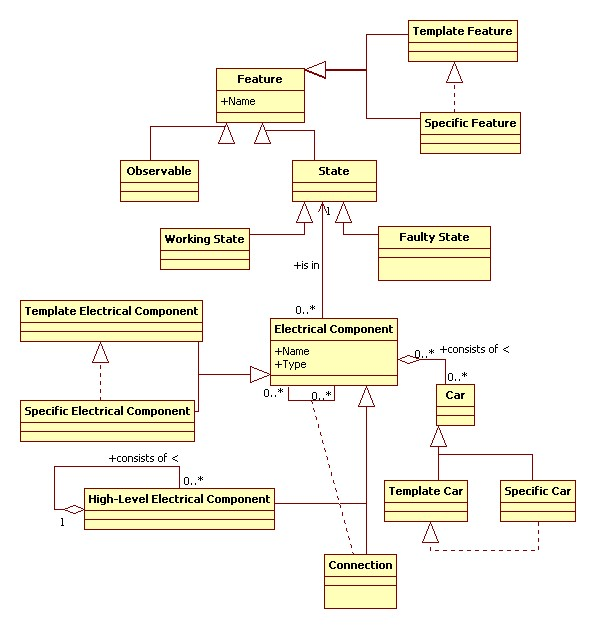
\includegraphics[width=1.00\textwidth]{DomainSchema.jpg}
	\caption{Domain schema for the car diagnoses task}
	\label{fig:DS}
\end{figure}

\begin{figure}[htbp]
	\centering
		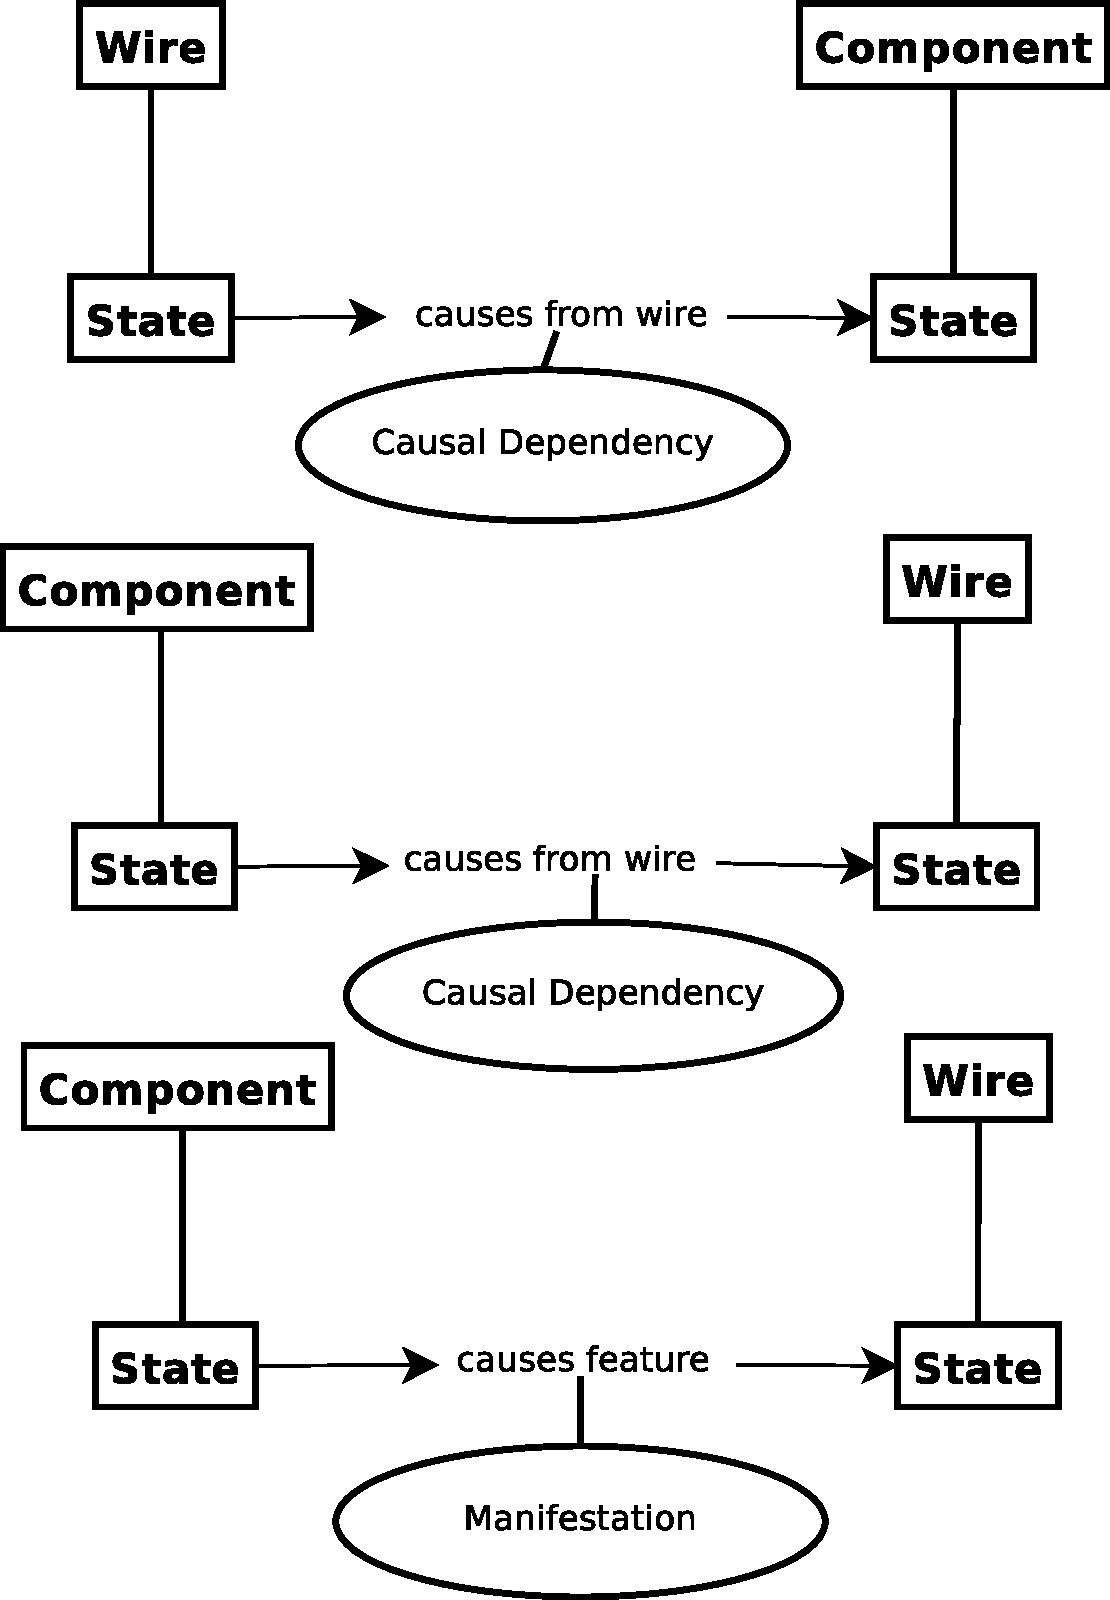
\includegraphics[width=1.00\textwidth]{rule-types.pdf}
	\caption{Rule types}
	\label{fig:IS}
\end{figure}

\subsubsection{Knowledge base}
Below is a general overview of our knowledge base. Because all rules together create a single causal model all rules are contained in a single knowledge base. Not all rules are shown. Instead we show one instance of every kind of rule and explain how the other rules look. This is done because the complete knowledge base is very large.

The CAUSES-TO-WIRE rules state that if a device is generating or passing through power and this device is in a state that makes it unable to perform this function then all wires leading from it will not be powered. A separate rule exists for the combinations of each device type with every possible state that would make it unable to power the wire.

\begin{verbatim}
KNOWLEDGE-BASE causal-model;
   USES:
      Component-knowledge
      Car-specific-knowledge
   EXPRESSIONS:
      A.state = empty
      A.type = battery
      B.type = connection
      B.comp1 = A
      CAUSES-TO-WIRE
      B.state = no-power
\end{verbatim}

\noindent
The CAUSES-FROM-WIRE rules state that if all wires connected to a device are in a state that makes them unable to pass on power then this device will not be powered. A separate rule exists for the combination of every wire state that makes the wire unable to pass on power and every device type.

\begin{verbatim}
      A.state = empty
      A.type = battery
      B.type = connection
      B.comp1 = A
      CAUSES-FROM-WIRE
      B.state = no-power
\end{verbatim}

\noindent
The CAUSES-FEATURE rules map states of actual devices to observables. A separate rule exists for the combination of every device with all of its possible states that cause an observable. Note that these rules are not general and are dependend on the car. Thus these rules represent specific car knowledge.

\begin{verbatim}
      A.name = head-light-left
      A.state = no-power
      CAUSES-FEATURE
      observable = head-light-left-no-light
END KNOWLEDGE-BASE causal-model;
\end{verbatim}


\subsubsection{Example of a car}
Figures~\ref{fig:ChargeSystem},~\ref{fig:LightSystem} and~\ref{fig:StartAndIgnitionSystem} show a graphical representation of an example car according to our model. This car consists of several electrical components. Normal electrical components are shown as objects in boxes with underlined text. Connections are, although they are objects as well, represented by arrows that show which components they connect. High level electrical components are shown as large boxes that contain other electrical components. Although the are represented in these diagrams they are not used in the reasoning process.

Note that the car is incomplete. It lacks, for example rear lights. The representation is based on a general notion of how cars work but it is not a (partial) representation of an existing car.

\begin{figure}[htbp]
	\centering
		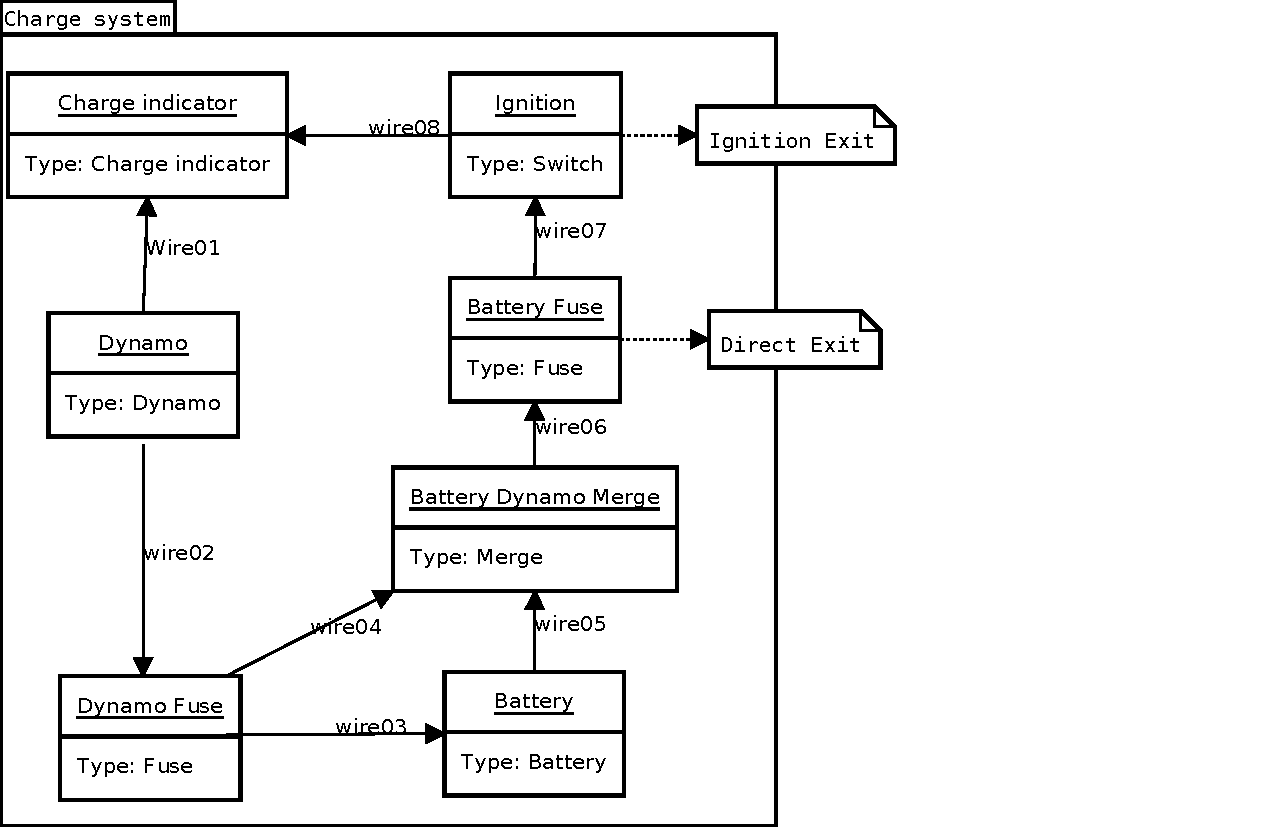
\includegraphics[width=1.00\textwidth]{ChargeSystem.pdf}
	\caption{The charge system of our example car}
	\label{fig:ChargeSystem}
\end{figure}

\begin{figure}[htbp]
	\centering
		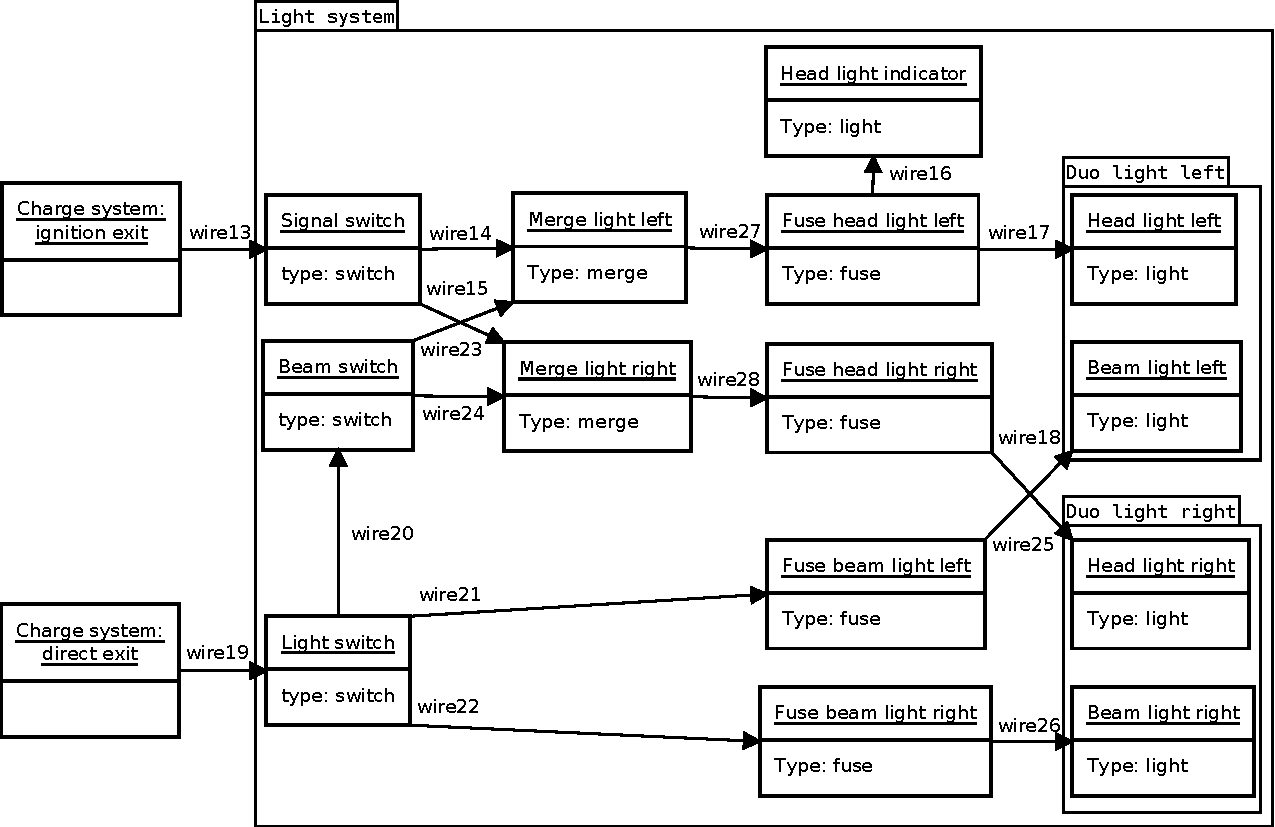
\includegraphics[width=1.00\textwidth]{LightSystem.pdf}
	\caption{The light system of our example car}
	\label{fig:LightSystem}
\end{figure}

\begin{figure}[htbp]
	\centering
		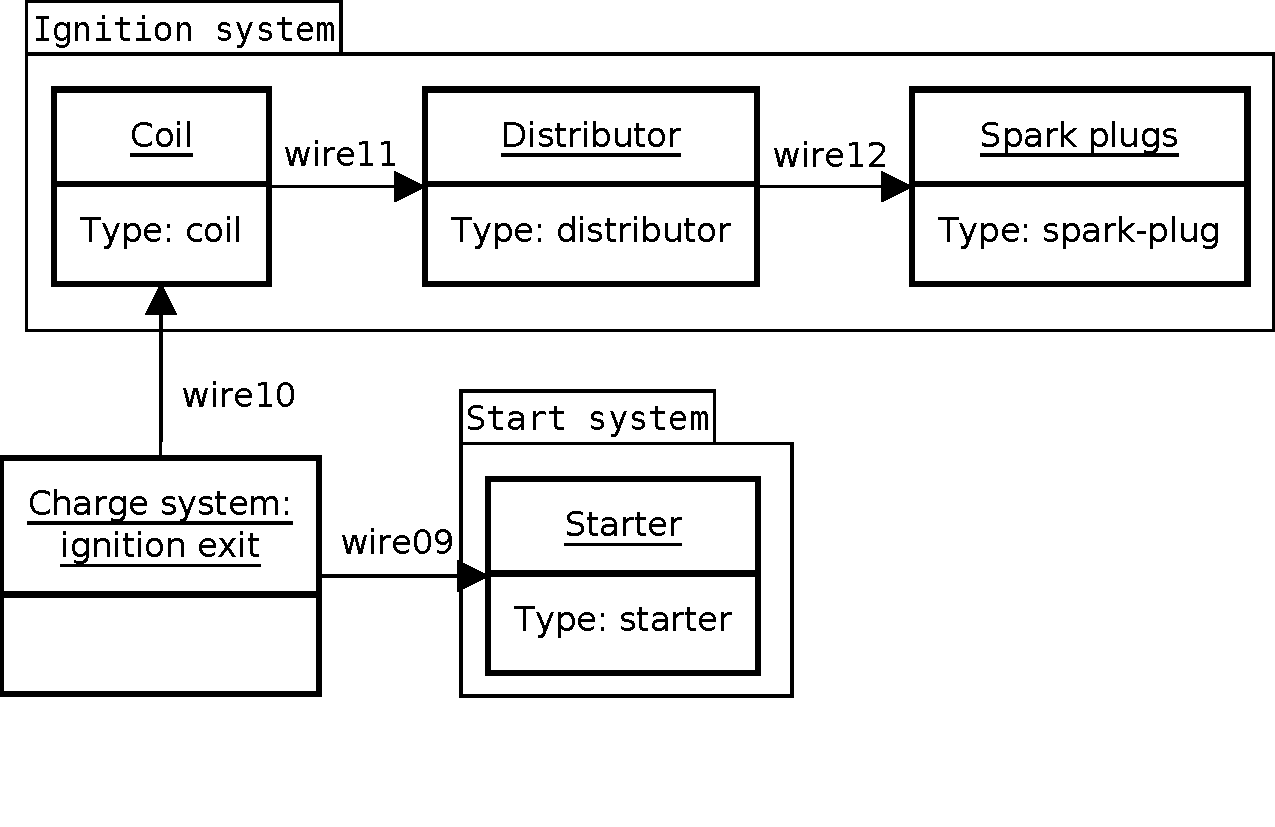
\includegraphics[width=1.00\textwidth]{StartAndIgnitionSystem.pdf}
	\caption{The start and the ignition system of our example car}
	\label{fig:StartAndIgnitionSystem}
\end{figure}


\subsection{Inference knowledge}
The inference model is shown in figure~\ref{fig:InferenceModel}. This inference model is almost exactly the same as the template shown in the common cads book. The only difference is an additional interaction with the user `obtain possible selection'. This interaction was added because our user would greatly like to influence the reasoning process by proposing his own hypothesis. The model is annotated with a simple example of how the system could work.

\begin{figure}[htbp]
	\centering
		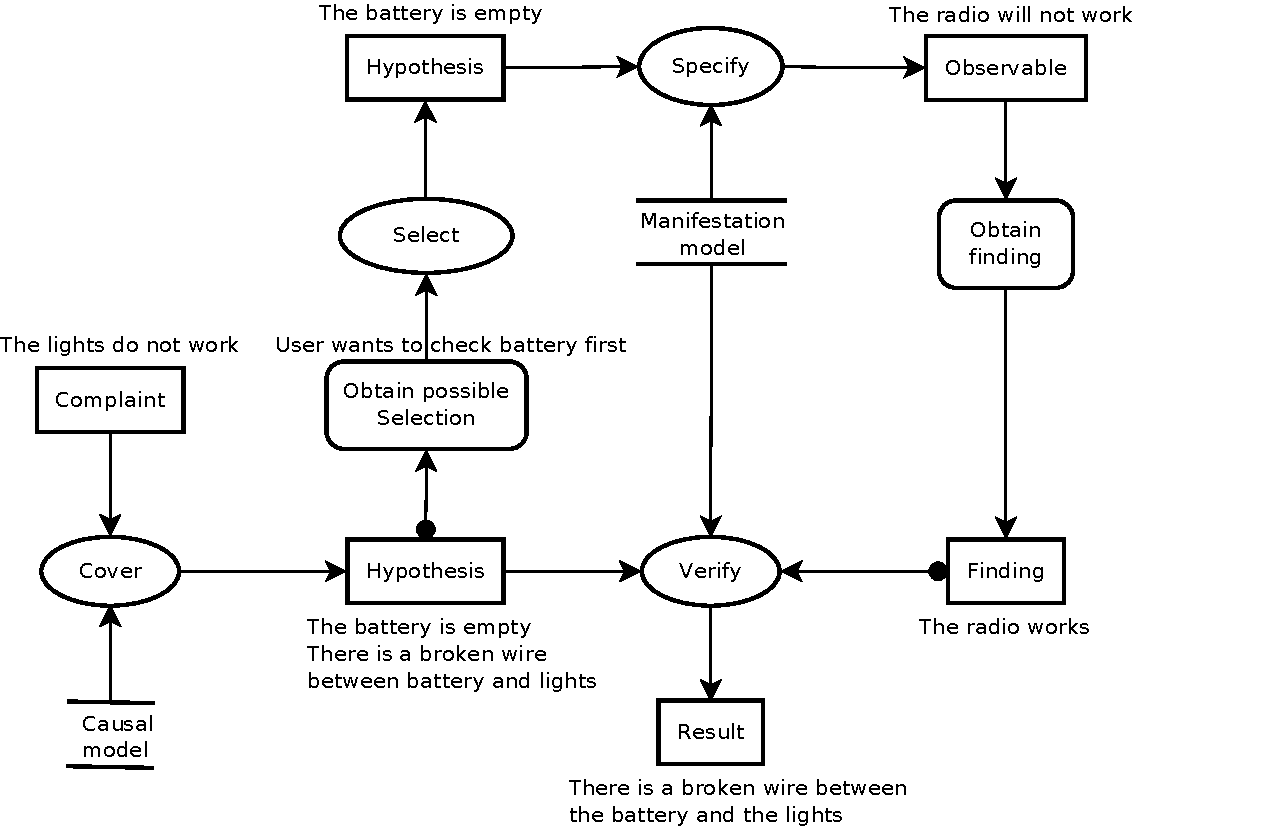
\includegraphics[width=1.00\textwidth]{inferenceModel.pdf}
	\caption{Annotated inference model}
	\label{fig:InferenceModel}
\end{figure}


\subsection{Task knowledge}
In our context analysis we identified to major task shown in the TM-1 tables. For this project we decided to focus only on the diagnoses task. The task model of the diagnoses task is shown in figure~\ref{fig:taskDecomposition}. The task model shows that the diagnoses task simply consists of the inference and interactions of the template diagnoses task plus the `obtain possible selection' interaction that we added to the template.

\begin{figure}[htbp]
	\centering
		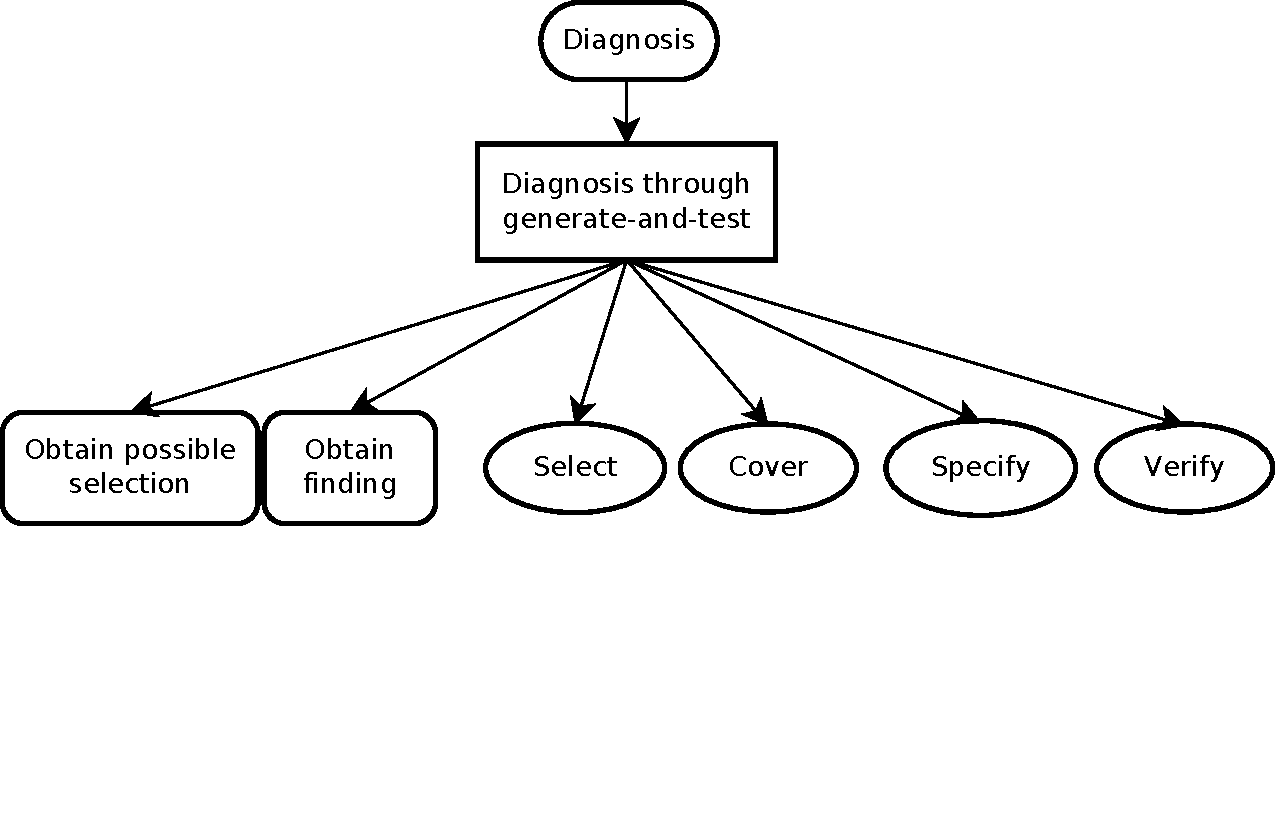
\includegraphics[width=1.00\textwidth, trim = 0 130 0 0, clip = true]{taskDecomposition.pdf}
	\caption{Task-decomposistion diagram for the diagnoses task}
	\label{fig:taskDecomposition}
\end{figure}


\section{Communication model}
Since our system is highly interactive the communication model is very important. Figure~\ref{fig:dialogueDiagram} shows all the transaction that exist between the system and the user. Most transaction are pretty straight forward consisting of just some data being send from one to the other. The negotiate observable transaction is more complex and it therefore has its own flow control shown in figure~\ref{fig:trans3-control}. More details about these transactions are shown in tables TM-1 and TM-2.

\subsection{CRA communication plan}
\begin{figure}[htbp]
	\centering
		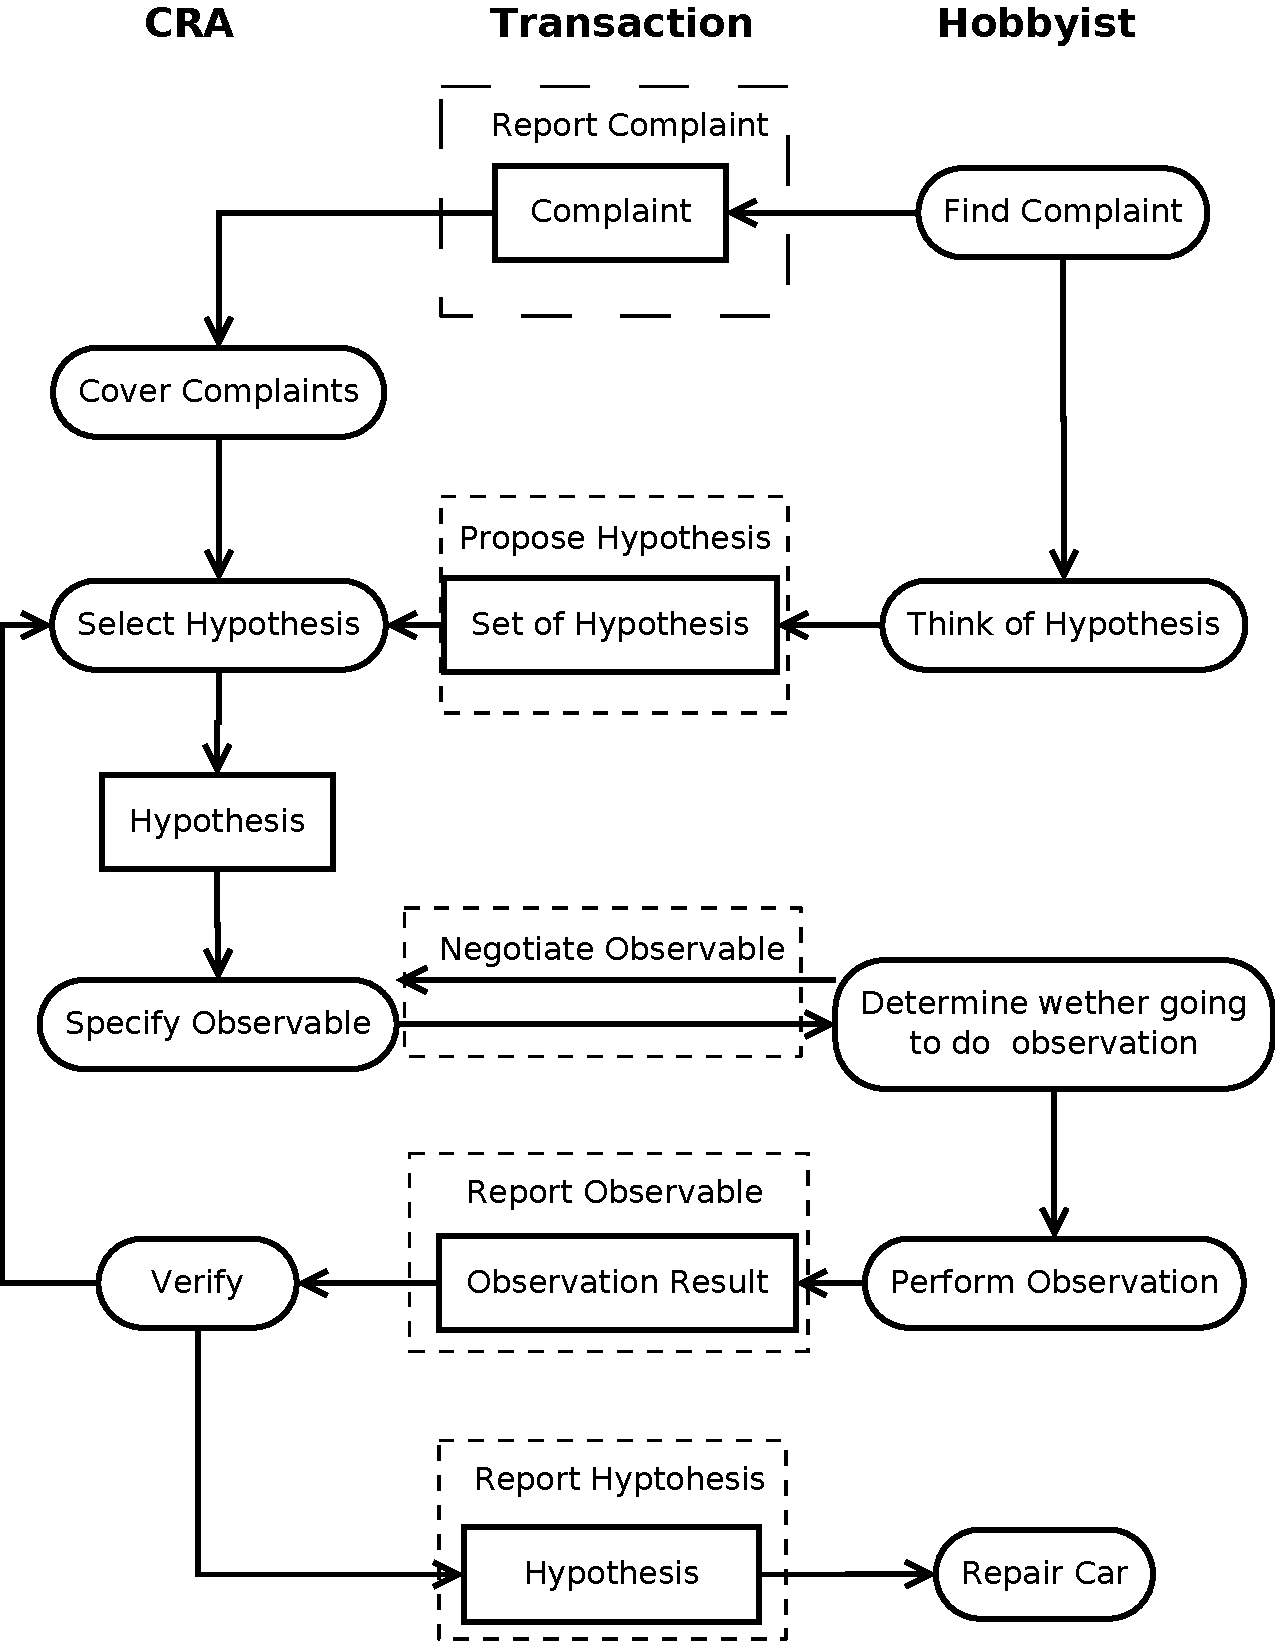
\includegraphics[width=1.00\textwidth]{dialogueDiagram.pdf}
	\caption{Dialogue diagram of the diagnoses task}
	\label{fig:dialogueDiagram}
\end{figure}

The control flow of the communication is shown in the communication plan (figure~\ref{fig:communicationPlan}). Because communication is so important in our system this plan is almost identical to the control flow of the CRA itself. 

As can be seen there is the need for a complaint at the start of the plan. Once this need is satisfied the state of the system will run in circles alternating between needing hypothesis, needing observables, found covering observations and observed observation until there are either no hypothesis or no observables left. At that point the plan is finished, either successful or unsuccessful.

\begin{figure}[htbp]
	\centering
		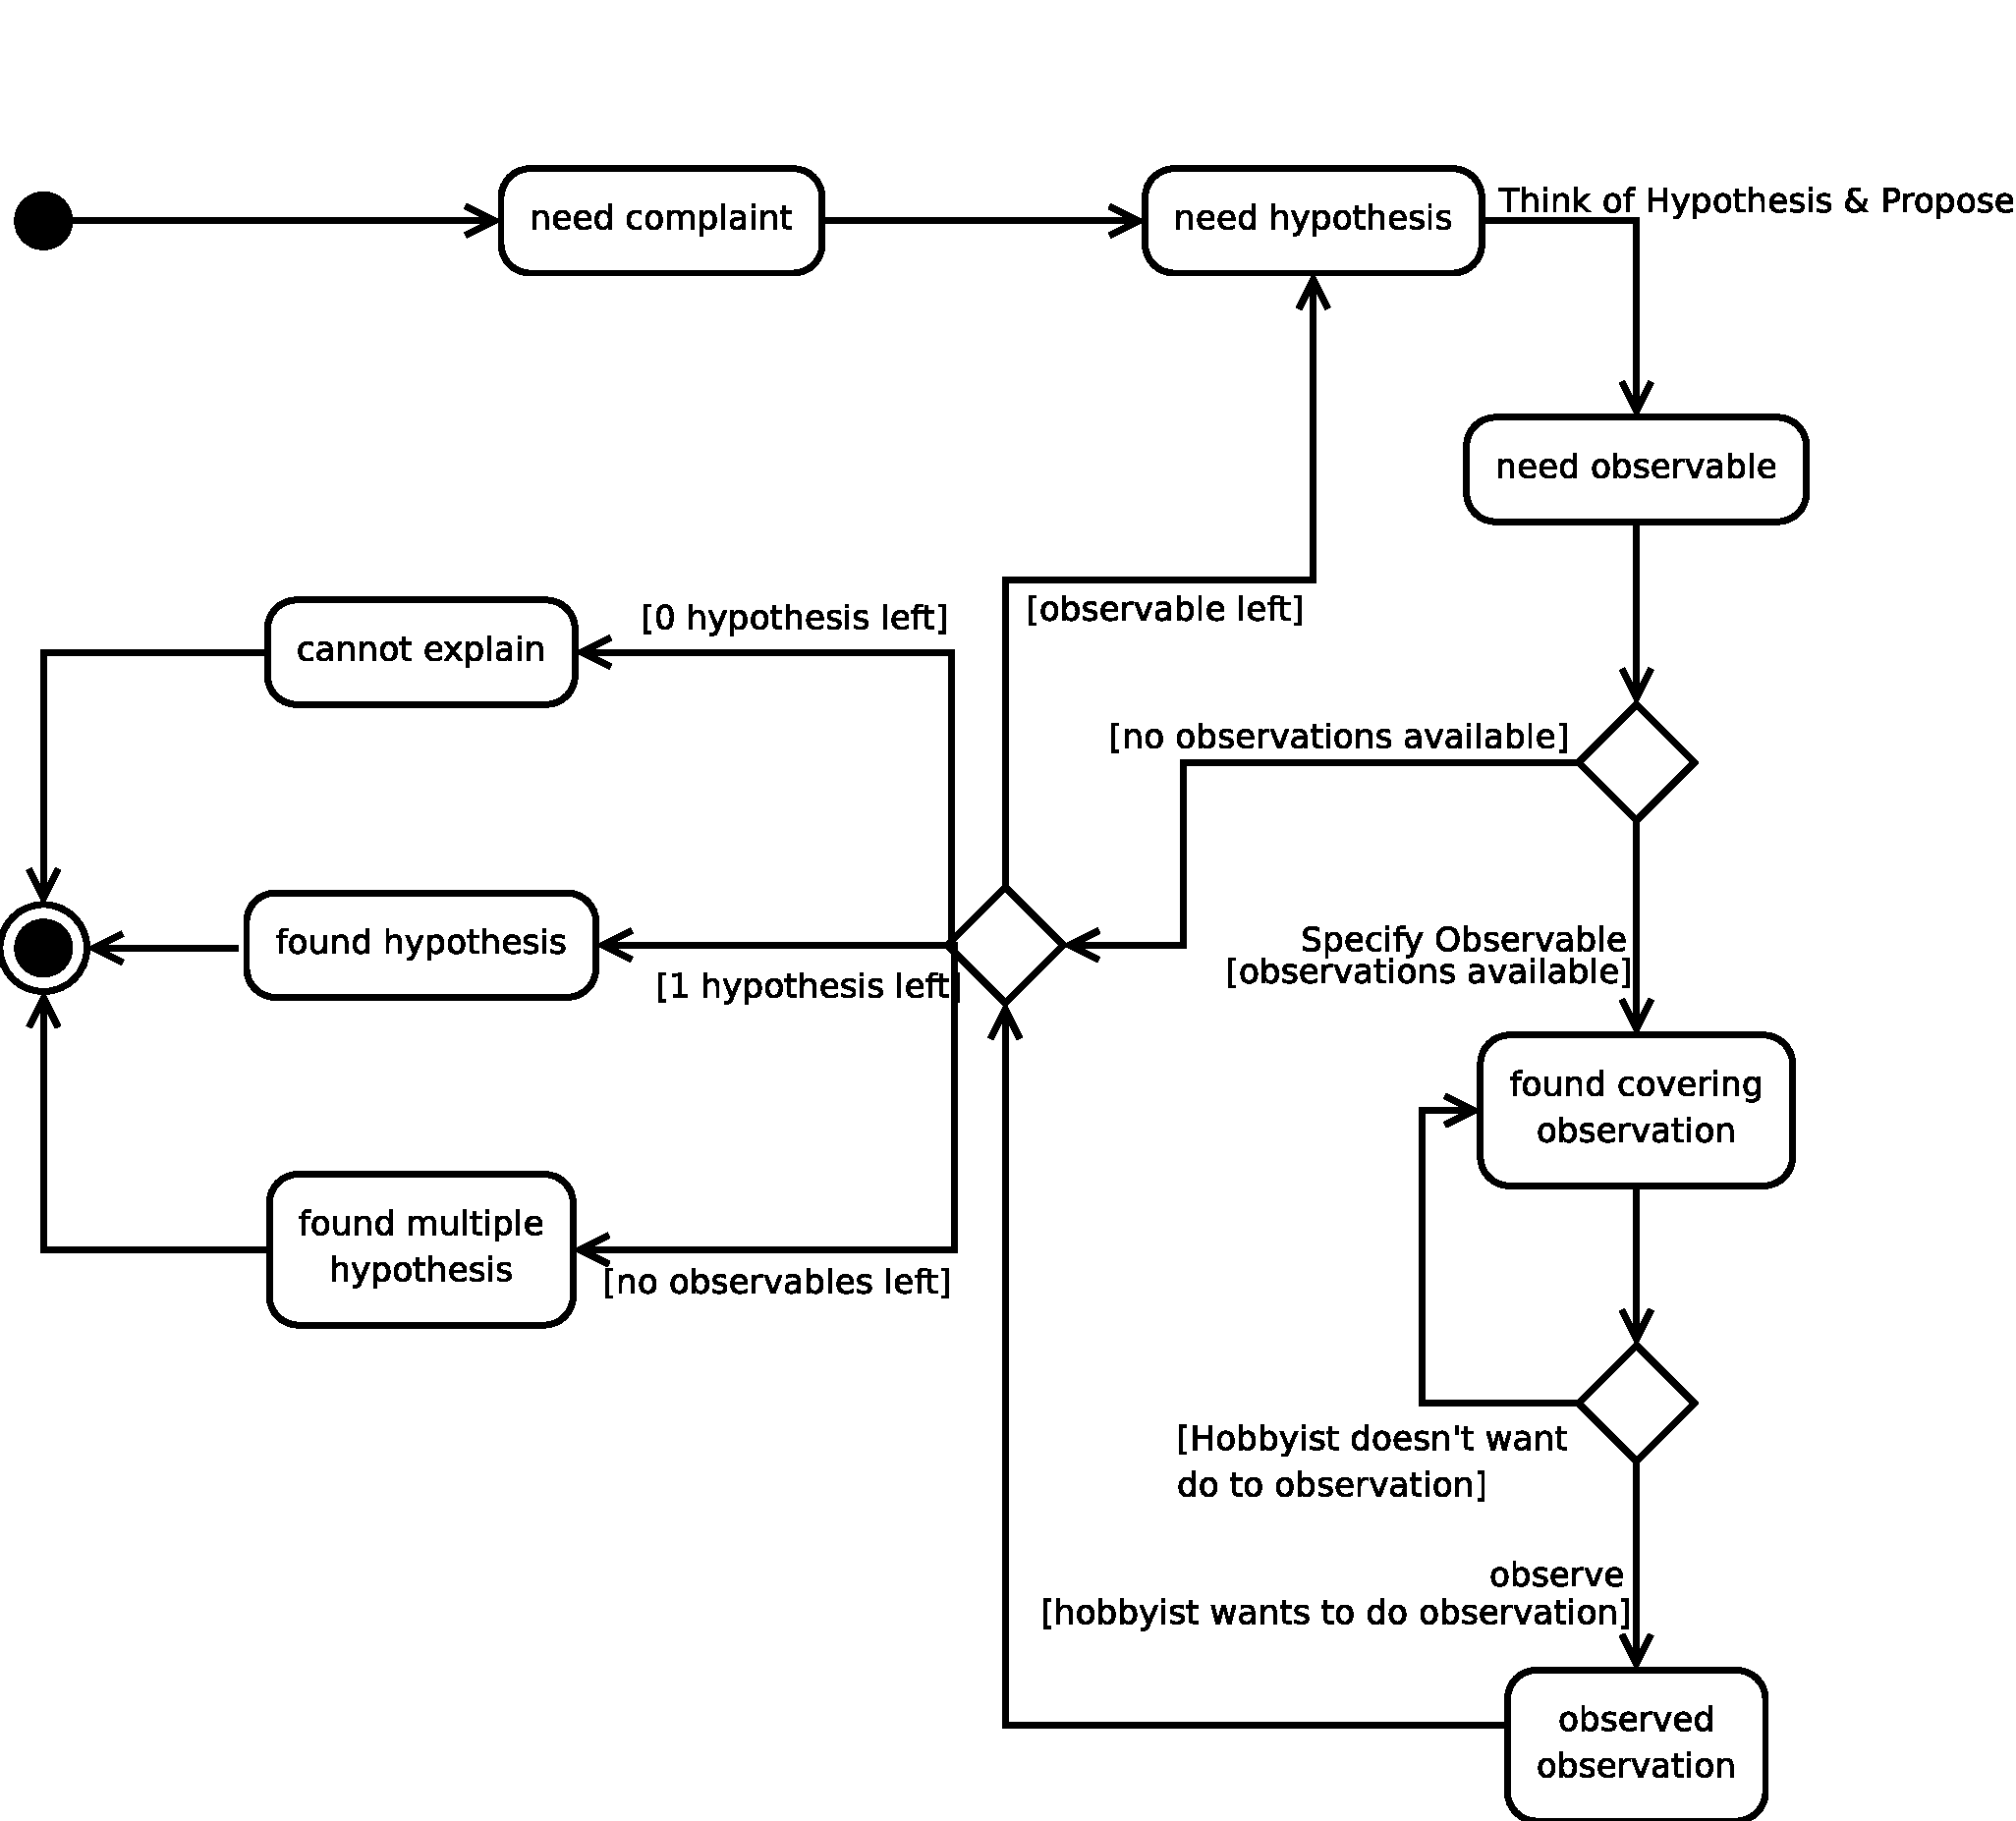
\includegraphics[width=1.00\textwidth]{communicationPlan.pdf}
	\caption{The communication plan of the diagnoses task.}
	\label{fig:communicationPlan}
\end{figure}

\subsection{CRA transactions}
% 1,2,5
\noindent
\begin{tabular}{%
       |>{\colleft}p{3cm}%
       |>{\colleft}p{8.5cm}|}
\hline
{\bf Communication model} &
   {\bf Transaction Description Worksheet CM-1} \\
\hline
\hline
\sc Transaction identifier/name &
	\emph{Transaction 1: Report complaint} \\

   %{\rm
   %A transaction is to be defined for each information object that is
   %output from some leaf task in the task model or in the knowledge
   %model (i.e., a transfer function), and that must be communicated to
   %another agent for use in its own tasks. The name must reflect, in a
   %user-understandable way, what is done with this information object
   %by the transaction. In addition to the name, give a brief
   %explanation here of the purpose of the transaction.
   %} 
\hline
\sc Information object &
	Transferring a complaint between the \emph{find complaint} and \emph{cover complaint} task. \\
   %{\rm
   %Indicate the (core) information object, and between which two
   %tasks it is to be transmitted.
   %} \\
\hline
\sc Agents involved &
	\emph{Car repair assistant}: receiving the complaint;\newline
	\emph{Hobbyist}: sending the complaint\\
   %{\rm
   %Indicate the agent that is sender of the information object,
   %and the agent that is receiving it.
   %} \\
\hline
\sc Communication plan &
	CRA communication plan\\

   %{\rm
   %Indicate the communication plan of which this transaction is a
   %component.
   %} \\
\hline
\sc Constraints &
	Before the transaction the car repair assistant must be ready to reiceve complaints\\

   %{\rm
   %Specify the requirements and (pre)conditions that must be fulfilled
   %so that the transaction can be carried out. Sometimes, it is also
   %useful to state post-conditions that are assumed to be valid after
   %the transaction.
   %} \\
\hline
\sc Information exchange specification &
	See worksheet CM-2 below.\\

   %{\rm
   %Transactions can have an internal structure, in that they consist
   %of several messages of different types, and/or handle additional
   %supporting information objects such as explanation or help items.
   %This is detailed in worksheet CM-2. At this point, only a reference
   %or pointer needs to be given to a later info exchange spec.
   %} \\
\hline
\end{tabular}


\noindent
\begin{tabular}{%
       |>{\colleft}p{3cm}%
       |>{\colleft}p{8.5cm}|}
\hline
{\bf Communication model} &
   {\bf Transaction Description Worksheet CM-1} \\
\hline
\hline
\sc Transaction identifier/name &
	\emph{Transaction 2: Propose hypothesis} \\

   %{\rm
   %A transaction is to be defined for each information object that is
   %output from some leaf task in the task model or in the knowledge
   %model (i.e., a transfer function), and that must be communicated to
   %another agent for use in its own tasks. The name must reflect, in a
   %user-understandable way, what is done with this information object
   %by the transaction. In addition to the name, give a brief
   %explanation here of the purpose of the transaction.
   %} 
\hline
\sc Information object &
	Transfering sets of hypothesis between the \emph{propose hypothesis} and \emph{select hypothesis} task. \\
   %{\rm
   %Indicate the (core) information object, and between which two
   %tasks it is to be transmitted.
   %} \\
\hline
\sc Agents involved &
	\emph{Hobbyist}: receiving the set of proposed hypothesis, sending a set of hypothesis (might be an empty set); \newline
	\emph{Car repair assistant}: sending a set of proposed hypothesis; receiving a set of hypothesis\\
   %{\rm
   %Indicate the agent that is sender of the information object,
   %and the agent that is receiving it.
   %} \\
\hline
\sc Communication plan &
	CRA communication plan\\

   %{\rm
   %Indicate the communication plan of which this transaction is a
   %component.
   %} \\
\hline
\sc Constraints &
	Before the transaction the car repair assistant must have a set of hypothesis ready. As a post condition one hypothesis has to be selected.\\

   %{\rm
   %Specify the requirements and (pre)conditions that must be fulfilled
   %so that the transaction can be carried out. Sometimes, it is also
   %useful to state post-conditions that are assumed to be valid after
   %the transaction.
   %} \\
\hline
\sc Information exchange specification &
	See worksheet CM-2 below.\\

   %{\rm
   %Transactions can have an internal structure, in that they consist
   %of several messages of different types, and/or handle additional
   %supporting information objects such as explanation or help items.
   %This is detailed in worksheet CM-2. At this point, only a reference
   %or pointer needs to be given to a later info exchange spec.
   %} \\
\hline
\end{tabular}

\noindent
\begin{tabular}{%
       |>{\colleft}p{3cm}%
       |>{\colleft}p{8.5cm}|}
\hline
{\bf Communication model} &
   {\bf Transaction Description Worksheet CM-1} \\
\hline
\hline
\sc Transaction identifier/name &
	\emph{Transaction 3: Negotiate observable} \\

   %{\rm
   %A transaction is to be defined for each information object that is
   %output from some leaf task in the task model or in the knowledge
   %model (i.e., a transfer function), and that must be communicated to
   %another agent for use in its own tasks. The name must reflect, in a
   %user-understandable way, what is done with this information object
   %by the transaction. In addition to the name, give a brief
   %explanation here of the purpose of the transaction.
   %} 
\hline
\sc Information object &
	Transferring observation instructions between the \emph{specify observable} and \emph{determine whether going to do observation} task. \\
   %{\rm
   %Indicate the (core) information object, and between which two
   %tasks it is to be transmitted.
   %} \\
\hline
\sc Agents involved &
	\emph{Car repair assistant}: sending observation instructions;\newline
	\emph{Hobbyist}: receiving observation instructions\\
   %{\rm
   %Indicate the agent that is sender of the information object,
   %and the agent that is receiving it.
   %} \\
\hline
\sc Communication plan &
	CRA communication plan\\

   %{\rm
   %Indicate the communication plan of which this transaction is a
   %component.
   %} \\
\hline
\sc Constraints &
	Before the transaction the car repair assistant must have a set of observables ready. As a post condition one observable must be excepted.\\

   %{\rm
   %Specify the requirements and (pre)conditions that must be fulfilled
   %so that the transaction can be carried out. Sometimes, it is also
   %useful to state post-conditions that are assumed to be valid after
   %the transaction.
   %} \\
\hline
\sc Information exchange specification &
	See worksheet CM-2 below.\\

   %{\rm
   %Transactions can have an internal structure, in that they consist
   %of several messages of different types, and/or handle additional
   %supporting information objects such as explanation or help items.
   %This is detailed in worksheet CM-2. At this point, only a reference
   %or pointer needs to be given to a later info exchange spec.
   %} \\
\hline
\end{tabular}


\noindent
\begin{tabular}{%
       |>{\colleft}p{3cm}%
       |>{\colleft}p{8.5cm}|}
\hline
{\bf Communication model} &
   {\bf Transaction Description Worksheet CM-1} \\
\hline
\hline
\sc Transaction identifier/name &
	\emph{Transaction 4: Report observable} \\

   %{\rm
   %A transaction is to be defined for each information object that is
   %output from some leaf task in the task model or in the knowledge
   %model (i.e., a transfer function), and that must be communicated to
   %another agent for use in its own tasks. The name must reflect, in a
   %user-understandable way, what is done with this information object
   %by the transaction. In addition to the name, give a brief
   %explanation here of the purpose of the transaction.
   %} 
\hline
\sc Information object &
	Transferring observation result between the \emph{perform observation} and \emph{verify} task. \\
   %{\rm
   %Indicate the (core) information object, and between which two
   %tasks it is to be transmitted.
   %} \\
\hline
\sc Agents involved &
	\emph{Hobbyist}: sending observation result;			\newline
	\emph{Car repair assistant}: receiving observation result	\\
   %{\rm
   %Indicate the agent that is sender of the information object,
   %and the agent that is receiving it.
   %} \\
\hline
\sc Communication plan &
	CRA communication plan\\

   %{\rm
   %Indicate the communication plan of which this transaction is a
   %component.
   %} \\
\hline
\sc Constraints &
	Before the transaction the hobbyist must have carried out the observation instructions and remembered there results.\\
   %{\rm
   %Specify the requirements and (pre)conditions that must be fulfilled
   %so that the transaction can be carried out. Sometimes, it is also
   %useful to state post-conditions that are assumed to be valid after
   %the transaction.
   %} \\
\hline
\sc Information exchange specification &
	See worksheet CM-2 below.\\

   %{\rm
   %Transactions can have an internal structure, in that they consist
   %of several messages of different types, and/or handle additional
   %supporting information objects such as explanation or help items.
   %This is detailed in worksheet CM-2. At this point, only a reference
   %or pointer needs to be given to a later info exchange spec.
   %} \\
\hline
\end{tabular}

\noindent
\begin{tabular}{|>{\colleft}p{3cm}|>{\colleft}p{8.5cm}|}
\hline
{\bf Communication model} &
   {\bf Transaction Description Worksheet CM-1} \\
\hline
\hline
\sc Transaction identifier/name &
	\emph{Transaction 5: Report hypothesis} \\

   %{\rm
   %A transaction is to be defined for each information object that is
   %output from some leaf task in the task model or in the knowledge
   %model (i.e., a transfer function), and that must be communicated to
   %another agent for use in its own tasks. The name must reflect, in a
   %user-understandable way, what is done with this information object
   %by the transaction. In addition to the name, give a brief
   %explanation here of the purpose of the transaction.
   %} 
\hline
\sc Information object &
	Transferring hypothesis result between the \emph{verify} and \emph{repair car} task. \\
   %{\rm
   %Indicate the (core) information object, and between which two
   %tasks it is to be transmitted.
   %} \\
\hline
\sc Agents involved &
	\emph{Car repair assistant}: sending hypothesis;	\newline
	\emph{Hobbyist}: receiving hypothesis			\\
   %{\rm
   %Indicate the agent that is sender of the information object,
   %and the agent that is receiving it.
   %} \\
\hline
\sc Communication plan &
	CRA communication plan\\

   %{\rm
   %Indicate the communication plan of which this transaction is a
   %component.
   %} \\
\hline
\sc Constraints &
	Before the transaction the car repair assistant must have either no observations left or he has one or less hypothesis left.\\
   %{\rm
   %Specify the requirements and (pre)conditions that must be fulfilled
   %so that the transaction can be carried out. Sometimes, it is also
   %useful to state post-conditions that are assumed to be valid after
   %the transaction.
   %} \\
\hline
\sc Information exchange specification &
	See worksheet CM-2 below.\\

   %{\rm
   %Transactions can have an internal structure, in that they consist
   %of several messages of different types, and/or handle additional
   %supporting information objects such as explanation or help items.
   %This is detailed in worksheet CM-2. At this point, only a reference
   %or pointer needs to be given to a later info exchange spec.
   %} \\
\hline
\end{tabular}
\noindent
\begin{tabular}{|>{\colleft}p{3cm}|>{\colleft}p{8.5cm}|} \hline
{\bf Communication model} 	& {\bf Information Exchange Specification Worksheet CM-2} \\ \hline \hline
\sc Transaction 			& \emph{Transaction 1: Report complaint}  \\ \hline
\sc Agents involved 		& 1. {\bf Sender}(Hobbyist): Initiate repair  \newline
					  2. {\bf Receiver}(Car repair assistant): Initiate repair \newline
					  3. {\bf Sender}(Car repair assistant): List of complaints  \newline
					  4. {\bf Receiver}(Hobbyist): List of complaints  \newline
					  5. {\bf Sender}(Hobbyist): Complaint  \newline
					  6. {\bf Receiver}(Car repair assistant): Complaint \\ \hline
\multicolumn{2}{|l|}{\textsc{Information items}} \\ \hline
   					%List all information items that are to be transmitted in this
   					%transaction. This includes the (`core') information object the
   					%transfer of which is the purpose of the transaction. However, it may contain
   					%other, supporting, information items, that, for example, provide help
   					%or explanation. For each information item, describe the following:
   
INITIATE REPAIR			&  1. {\bf Role}: A core information object. \newline
					% whether it is a {\em core} object, or a {\em support} item.
					   2. {\bf Form}: A signal indicating the start of a repair process \newline
					% the syntactic form in which it transmitted to another agent , e.g., data string, canned text, a certain type of diagram, 2D or 3D plot.
					   3. {\bf Medium}: By starting the program using an icon or command\\
					% the medium through which it is handled in the agent-agent interaction, e.g., a pop-up window, navigation and selection within a menu, command-line interface, human intervention.
LIST OF COMPLAINTS		&  1. {\bf Role}: A support information object. \newline
					   2. {\bf Form}: A list of strings \newline
					   3. {\bf Medium}: As menu items\\
COMPLAINT				&  1. {\bf Role}: A core information object. \newline
					   2. {\bf Form}: An identifier \newline
					   3. {\bf Medium}: As a selection within a menu\\ \hline
\multicolumn{2}{|l|}{\textsc{Message specifications}}\\ \hline
					% Describe all messages that make up the transaction. For each individual message describe:
INITIATION-MESSAGE		& {\bf Communication type}: ORDER\newline
					% the communication type of the message describing its intention (``illocutionary force,'' in speech-act terminology). 
					  {\bf Content}: Initiate repair\newline
					% the statement or proposition contained in the message.
					%&  3. {\bf Reference}: \\ \hline
					%in certain cases, it may be useful to add a reference to, for example, what domain knowledge model or agent capability is required to be able to send or process the message.
					  {\bf From}: Hobbyist\newline
					  {\bf To}: Car repair assistant\\
COMPLAINTS-LIST-MESSAGE		& {\bf Communication type}: REQUIRE\newline
					  {\bf Content}: List of complaints and the request to chose one\newline
					%&  3. {\bf Reference}: \newline
					  {\bf From}: Car repair assistant\newline
					  {\bf To}: Hobbyist\\
COMPLAINT-MESSAGE			& {\bf Communication type}: AGREE/REPORT\newline
					  {\bf Content}: Complaint\newline
					%&  3. {\bf Reference}: \\ \hline
					  {\bf From}: Hobbyist\newline
					  {\bf To}: Car repair assistant\\\hline
%\sc Control over messages 	& \\ \hline
   					%Give, if necessary, a control specification over the messages
   					%within the transaction. This can be done in pseudocode format or
   					%in a state-transition diagram, similar to how the control over
   					%transaction within the communication plan is specified. The
   					%difference is just the level of detail.
\end{tabular}

\noindent
\begin{tabular}{|>{\colleft}p{3cm}|>{\colleft}p{8.5cm}|} \hline
{\bf Communication model} 	& {\bf Information Exchange Specification Worksheet CM-2} \\ \hline \hline
\sc Transaction 			& \emph{Transaction 2: Propose hypothesis}  \\ \hline
\sc Agents involved 		& 1. {\bf Sender}(Car repair assistant): List of hypothesis  \newline
					  2. {\bf Receiver}(Hobbyist): List of hypothesis \newline
					  3. {\bf Sender}(Hobbyist): Hypothesis  \newline
					  4. {\bf Receiver}(Car repair assistant): Hypothesis \\ \hline
\multicolumn{2}{|l|}{\textsc{Information items}} \\ \hline
   					%List all information items that are to be transmitted in this
   					%transaction. This includes the (`core') information object the
   					%transfer of which is the purpose of the transaction. However, it may contain
   					%other, supporting, information items, that, for example, provide help
   					%or explanation. For each information item, describe the following:
LIST OF HYPOTHESIS		&  1. {\bf Role}: A support information object. \newline
					   2. {\bf Form}: A list of strings \newline
					   3. {\bf Medium}: As menu items\\
HYPOTHESIS				&  1. {\bf Role}: A core information object. \newline
					   2. {\bf Form}: An identifier \newline
					   3. {\bf Medium}: As a selection within a menu\\
\multicolumn{2}{|l|}{\textsc{Message specifications}}\\ \hline
					% Describe all messages that make up the transaction. For each individual message describe:
HYPOTHESIS-LIST-MESSAGE		& {\bf Communication type}: REQUIRE\newline
					  {\bf Content}: List of hypothesis and the request to chose one\newline
					%&  3. {\bf Reference}: \newline
					  {\bf From}: Car repair assistant\newline
					  {\bf To}: Hobbyist\\
HYPOTHESIS-MESSAGE		& {\bf Communication type}: AGREE/REPORT\newline
					  {\bf Content}: Hypothesis\newline
					%&  3. {\bf Reference}: \\ \hline
					  {\bf From}: Hobbyist\newline
					  {\bf To}: Car repair assistant\\
NO-HYPOTHESIS-MESSAGE		& {\bf Communication type}: REJECT-ta\newline
					  {\bf Content}: rejection \newline
					%&  3. {\bf Reference}: \\ \hline
					  {\bf From}: Hobbyist\newline
					  {\bf To}: Car repair assistant\\\hline
%\textsc{Control over messages}& See code below. \\ \hline
   					%Give, if necessary, a control specification over the messages
   					%within the transaction. This can be done in pseudocode format or
   					%in a state-transition diagram, similar to how the control over
   					%transaction within the communication plan is specified. The
   					%difference is just the level of detail.
\end{tabular}

%\begin{verbatim}
%SEND(COMPONENT-LIST-MESSAGE)
%REPEAT WHILE <no NO-HYPOTHESIS-MESSAGE received>
%  IF <user wants to suggest a hypothesis> 
%  THEN 
%    IF <COMPONENT-LIST-MESSAGE received> 
%    THEN 
%      SEND(COMPONENT-MESSAGE)
%    END-IF
%    IF <MALFUNCTION-LIST-MESSAGE received> 
%    THEN 
%      SEND(MALFUNCTION-MESSAGE)
%    END-IF
%  ELSE 
%    SEND NO-HYPOTHESIS-MESSAGE
%  END-IF
%  IF <COMPONENT-MESSAGE received>  
%  THEN 
%    SEND(MALFUNCTION-LIST-MESSAGE)
%  END-IF
%  IF <MALFUNCTION-MESSAGE received> 
%  THEN 
%    PROCESS(store-hypothesis)
%  END-IF
%END-REPEAT
%\end{verbatim}


\noindent
\begin{tabular}{ %
       |>{\colleft}p{4cm}%
       |>{\colleft}p{8.5cm}|}
\hline
{\bf Communication model} & {\bf Information Exchange Specification Worksheet CM-2} \\
\hline
\hline
{\sc Transaction} &
%   Give the transaction identifier and the name of which this information
%   exchange specification is a part.
Transaction 3: Negotiate Observable
 \\
\hline
{\sc Agents involved} &
1. {\bf Sender}
%agent sending the information item(s)
CRA send a request for an observation, and an explanation of that observation
\newline
2. {\bf Receiver}:
The hobbyist receives the request for an observation, and an explanation.
%agent receiving the information item(s)
\\
\hline
\multicolumn{2}{|l|}{\textsc{Information items}} \\ \hline
&  There are two information objects, the name of the observation to be done, and an
explanation of that observation. 
%   List all information items that are to be transmitted in this
%   transaction. This includes the (`core') information object the
%   transfer of which is the purpose of the transaction. However, it may contain
%   other, supporting, information items, that, for example, provide help
%   or explanation. For each information item, describe the following:
   \newline
  1. {\bf Role}: The name of the observation is core, while the explanation is
support.
%whether it is a core object, or a support item.
   \newline
  2. {\bf Form}: The name of the observation is a string. The explanation is
canned rich text.
     % the syntactic form in which it transmitted to
     % another agent , e.g., data string, canned text, a certain type of
     % diagram, 2D or 3D plot.
   \newline
  3. {\bf Medium}: The name of the observation can be selected in a menu. The
explanation can be shown in a text box.
     % the medium through which it is handled in the
     % agent-agent interaction, e.g., a pop-up window, navigation and
     % selection within a menu, command-line interface, human
     % intervention.
   \\
\hline
\multicolumn{2}{|l|}{\textsc{Message specifications}}\\ \hline
{\sc 1. REQUEST-OBSERVATION} &
   {\bf Communication type}: REQUEST \newline
   {\bf Content}: Request for some observation \newline
   {\bf From}: CRA \newline
   {\bf To}: The hobbyist \\
   
{\sc 2. OFFER-OBSERVATION} &
   {\bf Communication type}: OFFER \newline
   {\bf Content}: The Hobbyist wants to do a certain observation \newline
  {\bf From}: The hobbyist \newline
  {\bf To}: CRA \\
   
{\sc 3. DO-OBSERVATION} &
   {\bf Communication type}: ORDER \newline
  {\bf Content}: explanation and observation the hobbyist needs to make\newline
  {\bf From}: CRA \newline
  {\bf To}: The hobbyist \\
   
{\sc 4. REJECT-OBSERVATION-REQUEST} &
   {\bf Communication type}: REJECT-ta \newline
  {\bf Content}: Don't want to do this observation \newline
  {\bf From}: The hobbyist \newline
  {\bf To}: CRA \\
   
{\sc 5. REJECT-OBSERVATION-OFFER} &
   {\bf Communication type}: REJECT-td \newline
  {\bf Content}: Explanation why that observation is not needed \newline
  {\bf From}: CRA \newline
  {\bf To}: The hobbyist \\
   
\hline
\sc Control over messages &
    % Give, if necessary, a control specification over the messages
    % within the transaction. This can be done in pseudocode format or
    % in a state-transition diagram, similar to how the control over
    % transaction within the communication plan is specified. The
    % difference is just the level of detail.
    See figure~\ref{fig:trans3-control}.
   \\
\hline
\end{tabular}

\begin{figure}[htbp]
	\centering
		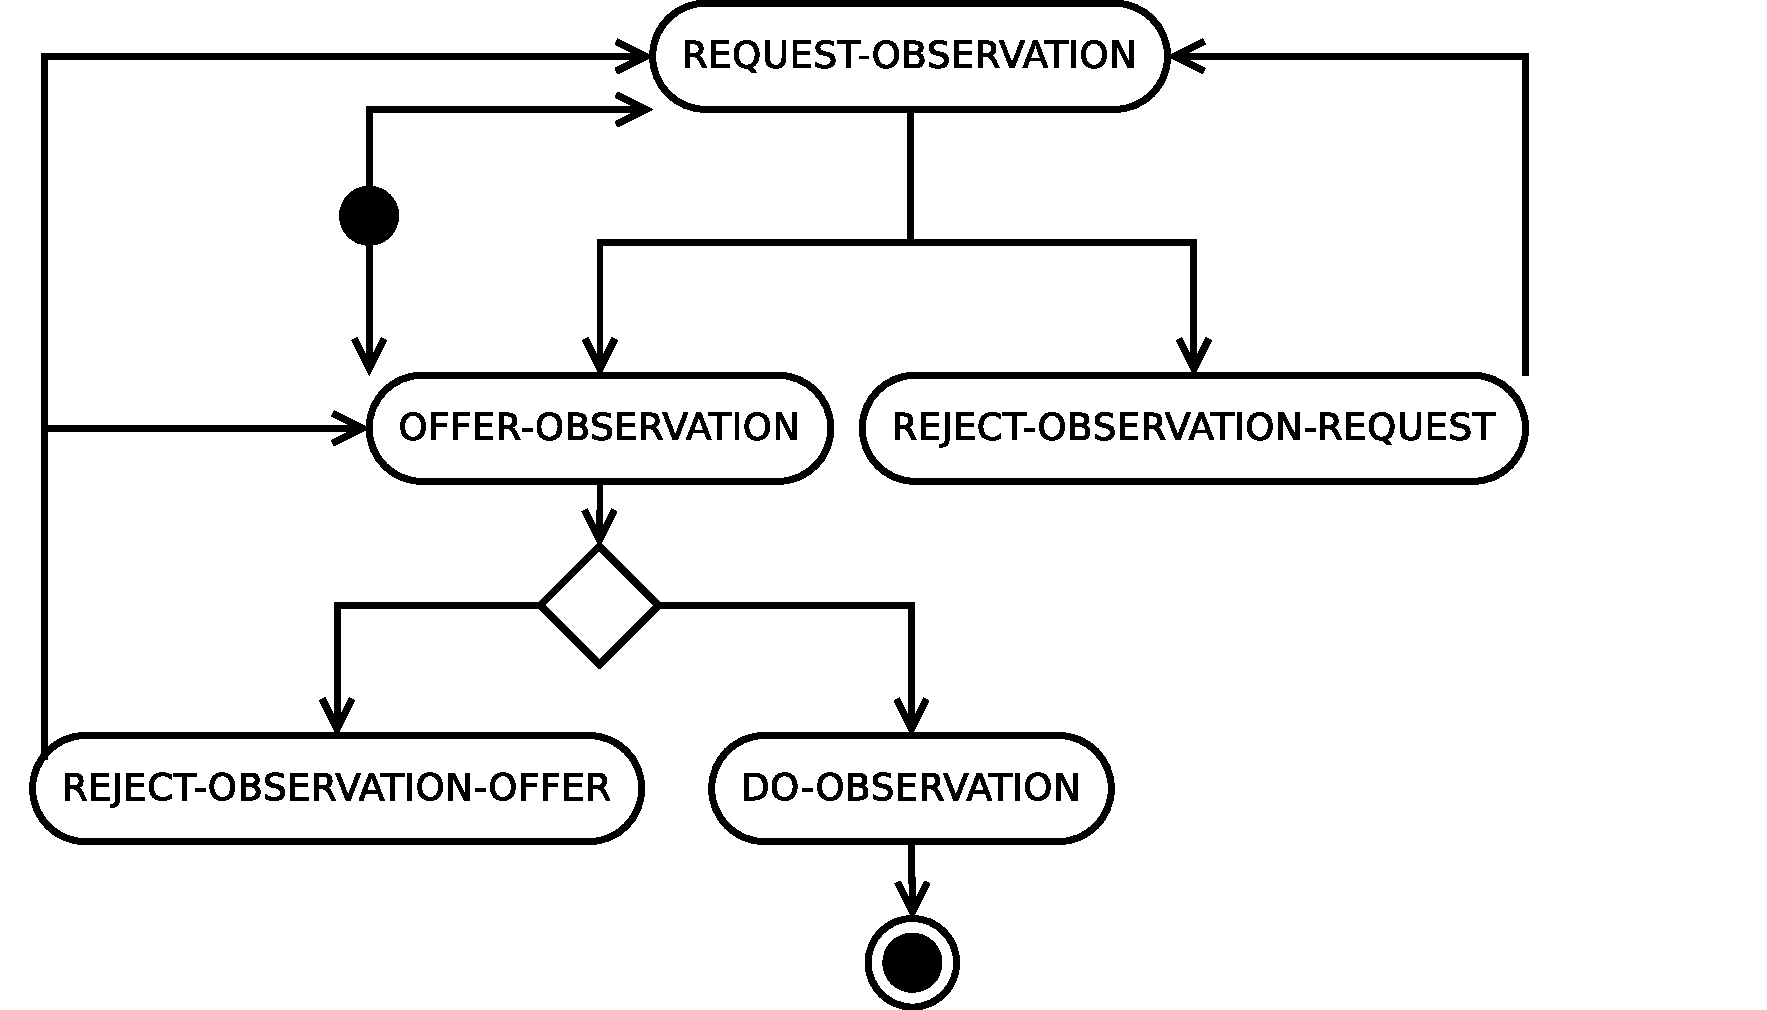
\includegraphics[width=1.00\textwidth]{trans3-control.pdf}
	\caption{Control flow of the negotiate observable transaction}
	\label{fig:trans3-control}
\end{figure}




\noindent
\begin{tabular}{|>{\colleft}p{3cm}|>{\colleft}p{8.5cm}|} \hline
{\bf Communication model} 	& {\bf Information Exchange Specification Worksheet CM-2} \\ \hline \hline
\sc Transaction 			& \emph{Transaction 4: Report observable} \\ \hline
\sc Agents involved 		& 1. {\bf Sender}(Car repair assistant): Observation result options  \newline
					  2. {\bf Receiver}(Hobbyist): Observation result options \newline
					  3. {\bf Sender}(Hobbyist): Observation result \newline
					  4. {\bf Receiver}(Car repair assistant): Observation result \\ \hline
					  
\multicolumn{2}{|l|}{\textsc{Information items}} \\ \hline
   					%List all information items that are to be transmitted in this
   					%transaction. This includes the (`core') information object the
   					%transfer of which is the purpose of the transaction. However, it may contain
   					%other, supporting, information items, that, for example, provide help
   					%or explanation. For each information item, describe the following:
OBSERVATION RESULT OPTIONS	&  1. {\bf Role}: A support information object. \newline
					% whether it is a {\em core} object, or a {\em support} item.
					   2. {\bf Form}: List of strings  \newline
					% the syntactic form in which it transmitted to another agent , e.g., data string, canned text, a certain type of diagram, 2D or 3D plot.
					   3. {\bf Medium}: Varies, it might be a menu or it might be a free form with suggestions noted separately\\ 
					% the medium through which it is handled in the agent-agent interaction, e.g., a pop-up window, navigation and selection within a menu, command-line interface, human intervention.
OBSERVATION RESULT		&  1. {\bf Role}: A core information object. \newline
					   2. {\bf Form}: Varies, it might be a identifier, a number or a string. \newline
					   3. {\bf Medium}: Varies, it might be selection in a menu or it might be typed in a field.\\ \hline
					
\multicolumn{2}{|l|}{\textsc{Message specifications}}\\ \hline
					% Describe all messages that make up the transaction. For each individual message describe:
OPTION-MESSAGE			& {\bf Communication type}: ASK \newline
					% the communication type of the message describing its intention (``illocutionary force,'' in speech-act terminology). 
					  {\bf Content}: Observation result options and the request to provide the actual observation result \newline
					% the statement or proposition contained in the message.
					% {\bf Reference}: car repair information\newline
					%in certain cases, it may be useful to add a reference to, for example, what domain knowledge model or agent capability is required to be able to send or process the message.
					  {\bf From}: Car repair assistant\newline
					  {\bf To}: Hobbyist\\ \hline
					  
OBSERVATION-MESSAGE		& {\bf Communication type}: REPLY \newline
					% the communication type of the message describing its intention (``illocutionary force,'' in speech-act terminology). 
					  {\bf Content}: The observation result \newline
					% the statement or proposition contained in the message.
					% {\bf Reference}: car repair information\newline
					%in certain cases, it may be useful to add a reference to, for example, what domain knowledge model or agent capability is required to be able to send or process the message.
					  {\bf From}: Hobbyist\newline
					  {\bf To}: Car repair assistant\\ \hline
%\sc Control over messages 	& \\ \hline
   					%Give, if necessary, a control specification over the messages
   					%within the transaction. This can be done in pseudocode format or
   					%in a state-transition diagram, similar to how the control over
   					%transaction within the communication plan is specified. The
   					%difference is just the level of detail.
\end{tabular}



\noindent
\begin{tabular}{|>{\colleft}p{3cm}|>{\colleft}p{8.5cm}|} \hline
{\bf Communication model} 	& {\bf Information Exchange Specification Worksheet CM-2} \\ \hline \hline
\sc Transaction 			& \emph{Transaction 5: Report hypothesis} \\ \hline
\sc Agents involved 		& 1. {\bf Sender}(Car repair assistant): Hypothesis  \newline
					  2. {\bf Sender}(Car repair assistant): Hypothesis argumentation \newline
					  3. {\bf Sender}(Car repair assistant): Repair plan \newline
					  4. {\bf Receiver}(Hobbyist): Hypothesis \newline
					  5. {\bf Receiver}(Hobbyist): Hypothesis argumentation \newline
					  6. {\bf Receiver}(Hobbyist): Repair plan \\ \hline
					  
\multicolumn{2}{|l|}{\textsc{Information items}} \\ \hline
   					%List all information items that are to be transmitted in this
   					%transaction. This includes the (`core') information object the
   					%transfer of which is the purpose of the transaction. However, it may contain
   					%other, supporting, information items, that, for example, provide help
   					%or explanation. For each information item, describe the following:
HYPOTHESIS				&  1. {\bf Role}: A core information object. \newline
					% whether it is a {\em core} object, or a {\em support} item.
					   2. {\bf Form}: A string stating the hypothesis \newline
					% the syntactic form in which it transmitted to another agent , e.g., data string, canned text, a certain type of diagram, 2D or 3D plot.
					   3. {\bf Medium}: Displayed in the main window\\ 
					% the medium through which it is handled in the agent-agent interaction, e.g., a pop-up window, navigation and selection within a menu, command-line interface, human intervention.
HYPOTHESIS ARGUMENTATION	&  1. {\bf Role}: A support information object. \newline
					   2. {\bf Form}: A list of strings each stating one reasoning step \newline
					   3. {\bf Medium}: Displayed in the main window\\
REPAIR PLAN				&  1. {\bf Role}: A support information object. \newline
					   2. {\bf Form}: A text, possibly with images\newline
					   3. {\bf Medium}: Displayed in the main window\\ \hline
					
\multicolumn{2}{|l|}{\textsc{Message specifications}}\\ \hline
					% Describe all messages that make up the transaction. For each individual message describe:
HYPOTHESIS-MESSAGE		& {\bf Communication type}: REPORT \newline
					% the communication type of the message describing its intention (``illocutionary force,'' in speech-act terminology). 
					  {\bf Content}: The hypothesis, the hypotheses argumentation and the repair plan (plan depending on car repair information)\newline
					% the statement or proposition contained in the message.
					  {\bf Reference}: car repair information\newline
					%in certain cases, it may be useful to add a reference to, for example, what domain knowledge model or agent capability is required to be able to send or process the message.
					  {\bf From}: Hobbyist\newline
					  {\bf To}: Car repair assistant\\ \hline
					  
%\sc Control over messages 	& \\ \hline
   					%Give, if necessary, a control specification over the messages
   					%within the transaction. This can be done in pseudocode format or
   					%in a state-transition diagram, similar to how the control over
   					%transaction within the communication plan is specified. The
   					%difference is just the level of detail.
\end{tabular}

\section{Reflection}
\subsection{The process}
The process of creating the knowledge based system went well in general.

There was a problem with, unsurprisingly, the contact with our expert. Although the expert, a student car technician, was chosen because he was more easily accessible then the average car mechanic it was still difficult to get an appointment. Because of this the initial domain schema was eventually created without the help of the expert. Also, since we initially waited for an appointment there was a great delayed in our project. The information that was eventually obtained through our expert could be added rather nicely to our domain knowledge, but this ordering undoubtedly influenced the final model.

We used most of the models and methods of CommonKADS during the project. The organization and agent
model is useful to define the boundary and context of the system. As the environment
of the system is very small, it only works together with the car hobbyist, we
quickly finished those. With the task model we could better define and narrow
down the task of the system. The knowledge model and the communication model
are very useful. They form the foundation of our implementation.

The knowledge
model makes clear what rules and inferences should be used by the system. It
also created problems which have disappeared when we implemented it. We struggled
with the
difference between inferences and rules types, designing a rule type for the
cover inference separately from a rule type for the verify and specify step. This
proved unnecessary when we implemented the rules.

The CRA needs to work together with the car hobbyist. Communication is essential
for the system. The communication model is great to model this. Creating this
model was time-consuming, but proved worthwhile.

We did try to make a design model based on the model view controller paradigm.
It was very unclear how this should be done. With little time left and good
preceding models we decided to just start the implementation based on the
knowledge and communication model. We implemented the causal rules and component
knowledge from the knowledge model in Jess. These rules were used in the
inferences that we also implemented in Jess. The control of the program is based
on the communication plan and dialog diagram of the communication model and
implemented in Java.

\subsection{The final result}
The Car Repair Assistant performs its tasks reasonably well. It gives all possible causes and it will slowly reduce the number of possible causes by querying the user about various observables. The user can also steers this process by giving suggestion about which causes should be examined next. The system is also very flexible and using it with an other car, or even an other electrical system is very simple. Nevertheless, there are a lot of possible improvements.

First, the Car Repair Assistant does not reason well over so called merges. These merges are places where two wires power a single component. When reasoning, if there exists an observation of a working component, and this component is powered only by a merge then there is the conclusion that the merge can not be unpowered. However, the system can not assign truth values for the connections powering the merge because either one might still be unpowered. As a result these hypothesis remain in the list of possible hypothesis. This makes the reasoning process much less powerful.

An other important point that could be improved upon is the method that the CRA uses to suggest hypothesis and observables. Right now it just choses one without any preferences. It would be a lot better if these would be selected based upon the ease of obtaining the observations or based upon the information gain.

A last obvious point of improvement would be in the interface. This system would be much more practical if it worked with a transparent picture of a car that depicted all the components and there locations. This would make the tool a lot easier to use for the users.

Unfortunately there was little time to create the implementation of the final Car Repair Assistant. This is part due to the delay at the start of our project and part due to the fact that two months is not very long to create a fully functional knowledge system.


\end{document}

